\documentclass[10pt]{beamer}
\usepackage[spanish]{babel}
\usepackage[latin1]{inputenc}
\usepackage{subfigure}
\usetheme{Warsaw} 
\usecolortheme{rose}
\useoutertheme{shadow}
\useinnertheme{rectangles}
\setbeamertemplate{navigation symbols}{}

\newtheorem{dfn}{Definici\'on}

\title[Modelos no lineales para el procesamiento de im\'agenes]{Paquete de Python para el procesamiento de im\'agenes usando varios modelos no lineales}
\author[Carlos Toledo Silva]{{Carlos Toledo Silva}\\
	{\and} \\
	{Tutor} \\
	MSc. Damian Vald\'es Santiago}
\institute{Universidad de La Habana}

\date{13 de diciembre 2022}

\begin{document}

	\frame{\titlepage}
	
	\begin{frame}
		\frametitle{Introducci\'on -- Surgimiento de los Modelos no Lineales}
		
		Puntos claves:
		
		\begin{itemize}
			\item El Procesamiento Lineal Cl\'asico de Im\'agenes tiene limitaciones.
			\item Oppenheim (1965) introduce la teor\'ia homom\'orfica.
			\item Jourlin y Pinoli (1988) proponen el primer modelo logar\'itmico para el procesamiento de im\'agenes.
			\item Patrascu y Buzuloiu (2001) proponen un modelo logar\'itmico sim\'etrico.
			\item Vertan y colaboradores (2008) proponen el modelo pseudo-logar\'itmico. 
			\item Diversas aplicaciones: correcci�n de iluminaci�n, mejora de contraste, mejora de imagen en color, ecualizaci�n de histogramas, mejora de rango din�mico, detecci�n de bordes, etc.
		\end{itemize}
		
	\end{frame}

	\begin{frame}
		\frametitle{Introducci\'on -- Objetivos}
		
		Objetivos:
		
		\begin{itemize}
			\item  Dise�o e implementaci�n de un m�dulo de Python donde se encuentren los modelos no lineales para el procesamiento de im�genes abordados en este trabajo.
			\item  Evaluaci�n de los diferentes modelos en cuanto a las
			diferentes operaciones, tipos de im�genes y situaciones.
		\end{itemize}
	
		Tareas de investigaci\'on:
		
		\begin{itemize}
			\item Revisar la literatura referente a los modelos no lineales para el procesamiento de im\'agenes.
			\item Implementaci\'on en Python de los diferentes modelos a partir de la bibliograf\'ia consultada.
			\item Creaci\'on de \textit{datasets} con diferentes tipos de im\'agenes para evaluar los modelos.
			\item Selecci\'on de m\'etricas para la evaluaci\'on de los modelos.
			\item Evaluaci\'on de los modelos.
			\item Arribar a conclusiones sobre la eficacia y utilidad de estos modelos. 
		\end{itemize}
		
	\end{frame}

	\begin{frame}
		\frametitle{Estado del Arte -- Conceptos}
		
		Conceptos relacionados a estos modelos:
		\begin{enumerate}
			\item M: L\'imite superior del rango de niveles de gris. Ej: $[0,M)$.
			
			\item Dominio: $E\subseteq \mathbb{R}$.
			
			\item Funci\'on de cambio a tonos de gris. 
			
			\item Funci\'on de cambio a niveles de gris.
			
			\item Suma: $v_1\oplus v_2$.
			
			\item Multiplicaci\'on por un escalar: $\lambda \otimes v$.
			
			\item Resta: $v_1 \ominus v_2$.
			
			\item Funci\'on del isomorfismo: $\varphi: E\to F,~ F\subseteq \mathbb{R}$.
			
			\item Inversa de la funci\'on del isomorfismo: $\varphi^{-1}: F\to E$.
		\end{enumerate}
	\end{frame}

	\begin{frame}
		\frametitle{Estado del Arte -- Modelo LIP}
		
		Nombre: Modelo Logar\'itmico Cl\'asico para el Procesamiento de Im\'agenes.
		
		Propuesto por: Jourlin y Pinoli (1988).
		
		Dominio: $E=[0,M) \lor E=(-\infty,M)$.
		
		Funci\'on de cambio a tonos de gris: $v=M-u$. 
		
		Funci\'on de cambio a niveles de gris: $u=M-v$.
		
		Suma: $v_1\oplus v_2=v_1+v_2-\frac{v_1v_2}{M}$.
		
		Multiplicaci\'on por un escalar: $\lambda \otimes v = M - M\left(1-\frac{v}{M}\right)^\lambda$.
		
		Opuesto: $\ominus v=-\frac{v}{1-\frac{v}{M}}$.
		
		Resta: $v_1 \ominus v_2 = \frac{v_1-v_2}{1-\frac{v_2}{M}}$.
		
		Funci\'on del isomorfismo: $\varphi(v) = -M\ln\left(1-\frac{v}{M}\right)$.
		
		Inversa de la funci\'on del isomorfismo: $\varphi^{-1} (x) = M\left(1-e^{-\frac{x}{M}}\right)$.\newline
		
		Si $E=[0,M)$ entonces $(E,\mathbb{R}^+, \oplus, \otimes)$ es un cono positivo.
		
		Si $E=(-\infty,M)$ entonces $(E, \mathbb{R}, \oplus, \otimes)$ es un espacio vectorial.
	\end{frame}

	\begin{frame}
		\frametitle{Estado del Arte -- Modelo HLIP}
		
		Nombre: Modelo Logar\'itmico Homom\'orfico para el Procesamiento de Im\'agenes.
		
		Propuesto por: Patrascu y Buzuloiu (2001).
		
		Dominio: $E = (-1, 1)$.
		
		Funci\'on de cambio a tonos de gris: $v=\frac{2}{M}\left(u-\frac{M}{2}\right)$.
		
		Funci\'on de cambio a niveles de gris: $u=\frac{M}{2}(v+1)$.
		
		Suma: $	v_1 \oplus v_2=\frac{v_1+v_2}{1+v_1v_2}$.
		
		Multiplicaci\'on por un escalar: $\lambda \otimes v =\frac{(1+v)^\lambda-(1-v)^\lambda}{(1+v)^\lambda+(1-v)^\lambda},~\lambda\in \mathbb{R}$.
		
		Opuesto: $\ominus v=-v$.
		
		Resta: $v_1\ominus v_2=\frac{v_1-v_2}{1-v_1v_2}$.
		
		Funci\'on del isomorfismo: $\varphi(v)=\frac{1}{2}\ln\left(\frac{1+v}{1-v}\right)$.
		
		Inversa de la funci\'on del isomorfismo: $\varphi^{-1}(x)=\frac{e^{2x}-1}{e^{2x}+1}$.\newline
		
		La estructura $(E, \mathbb{R}, \oplus, \otimes)$ es un espacio vectorial.
	\end{frame}
	
	\begin{frame}
		\frametitle{Estado del Arte -- Modelo PSLIP}
		
		Nombre: Modelo Pseudo-logar\'itmico para el Procesamiento de Im\'agenes.
		
		Propuesto por: Vertan y colaboradores (2008).
		
		Dominio: $E = [0, 1)$.
		
		Funci\'on de cambio a tonos de gris: $v = \frac{u}{M}$.
		
		Funci\'on de cambio a niveles de gris:  $u=M\cdot v$.
		
		Suma: $v_1\oplus v_2=\frac{v_1 + v_2 - 2v_1v_2}{1-v_1v_2}$.
		
		Multiplicaci\'on por un escalar: $\lambda \otimes v = \frac{\lambda v}{1+(\lambda-1)v},~\lambda\in \mathbb{R}^+$.
		
		Resta: $v_1\ominus v_2=\frac{v_1-v_2}{1+v_1v_2-2v_2}: v_1\geq v_2$.
		
		Funci\'on del isomorfismo: $\varphi(v)=\frac{v}{1-v}$.
		
		Inversa de la funci\'on del isomorfismo: $\varphi^{-1}(x)=\frac{x}{1+x}$.\newline
		
		La estructura $(E,\mathbb{R}^+, \oplus, \otimes)$ es un cono positivo. La extensi�n a un espacio vectorial se puede lograr mediante el uso de la funci�n generadora definida en $(-1,1)\to (-\infty,+\infty): \varphi(v)=\frac{v}{1-|v|}$.
	\end{frame}

	\begin{frame}
		\frametitle{Estado del Arte -- Modelo PLIP}
		
		Nombre: Modelo Logar\'itmico Parametrizado para el Procesamiento de Im\'agenes.
		
		Propuesto por: Panetta y colaboradores (2010).
		
		Funci\'on de cambio a tonos de gris: $v=\mu(M)-u$.
		
		Funci\'on de cambio a niveles de gris: $u=\mu(M)-v$.
		
		Suma: $v_1\oplus v_2=v_1+v_2-\frac{v_1v_2}{\gamma(M)}$.
		
		Multiplicaci\'on por un escalar: $c\otimes v=\gamma(M)-\gamma(M)(1-\frac{v}{\gamma(M)})^c$.
		
		Opuesto: $\ominus v=-\frac{v}{1-\frac{v}{\gamma(M)}}$.
		
		Resta: $v_1\ominus v_2=\frac{v_1-v_2}{1-\frac{v_2}{k(M)}}$.
		
		Funci\'on del isomorfismo: $\varphi(v)=-\lambda(M)\ln^\beta(1-\frac{v}{\lambda(M)})$.
		
		Inversa de la funci\'on del isomorfismo: $\varphi^{-1}(x)=\lambda(M)(1-(e^{-\frac{x}{\lambda(M)}})^{\frac{1}{\beta}})$.
	\end{frame}

	\begin{frame}
		\frametitle{Estado del Arte -- Modelo SLIP}
		
		Nombre: Modelo Logar\'itmico Sim\'etrico para el Procesamiento de Im\'agenes.
		
		Propuesto por: Navarro y colaboradores (2013).
		
		Dominio: $E=(-M,M)$.
		
		Suma: $	v_1\oplus v_2=M\cdot sgn(v_1+v_2)\left[1-\left(1-\frac{|v_1|}{M}\right)^{\gamma_1}\left(1-\frac{|v_2|}{M}\right)^{\gamma_2}\right],$
		
		$\gamma_1=\frac{sgn(v_1)}{sgn(v_1+v_2)},~\gamma_2=\frac{sgn(v_2)}{sgn(v_1+v_2)}$.
		
		Multiplicaci\'on por un escalar: $\lambda \otimes v = M\cdot sgn(\lambda v)\left[1-\left(1-\frac{|v|}{M}\right)^{|\lambda|}\right]$, $\lambda\in\mathbb{R}$.
		
		Opuesto: $\ominus v = (-1)\otimes v$.
		
		Resta: $v_1\ominus v_2=v_1\oplus(-1)\otimes v_2$.
		
		Funci\'on del isomorfismo: $\varphi(v)=-M\cdot sgn(v)\ln\left(1-\frac{|v|}{M}\right)$.
		
		Inversa de la funci\'on del isomorfismo: $\varphi^{-1}(x)=M\cdot sgn(x)\left(1-e^{-\frac{|x|}{M}}\right)$.\newline
		
		La estructura $(E, \mathbb{R}, \oplus, \otimes)$ es un espacio vectorial.
	\end{frame}

	\begin{frame}
		\frametitle{Propuesta -- Modelo PPSLIP}
		
		Nombre: Modelo Pseudo-logar\'itmico Parametrizado para el Procesamiento de Im\'agenes.
		
		\begin{block}{Versi\'on inicial: Parametrizar las funciones de cambio}
			Se parametrizan solo las funciones de cambio de la siguiente forma:
			\begin{equation*}
				v=\frac{u}{\delta(M)},~u=\delta(M)v 
			\end{equation*}
			tal que $\delta(M) \geq M$ y se mantienen el resto de operaciones del modelo PSLIP.
			
			Ventaja: Se parametriza el modelo para evitar la p\'erdida de informaci\'on.
			Desventaja: Las operaciones se parametrizan con el mismo par\'ametro. 
		\end{block}
	\end{frame}

	\begin{frame}
		\frametitle{Propuesta -- Modelo PPSLIP}
		\begin{block}{Versi\'on final: Eliminar las funciones de cambio y hacer los cambios directamente en las operaciones.}
			
			Suma: $u_1\oplus u_2=\frac{u_1+u_2-\frac{2u_1u_2}{\gamma(M)}}{1-\frac{u_1u_2}{\gamma(M)^2}}$.
			
			Multiplicaci\'on por un escalar: $c\otimes u=\frac{cu}{1+\frac{(c-1)u}{\gamma(M)}}$.
			
			Resta: $	u_1\ominus u_2=\frac{u_1-u_2}{1+\frac{u_1u_2}{k(M)^2}-\frac{2u_2}{k(M)}}: u_1\geq u_2$.
			
			Funci\'on del isomorfismo: $\varphi(u)=\frac{u}{\lambda(M)-u}$.
			
			Inversa de la funci\'on del isomorfismo: $\varphi^{-1}(x)=\lambda(M)\frac{x}{1+x}$.
		\end{block}
	\end{frame}

	\begin{frame}
		\frametitle{Propuesta -- M\'odulo Implementado -- Estructuras}
		
		\begin{figure}
			\begin{center}
				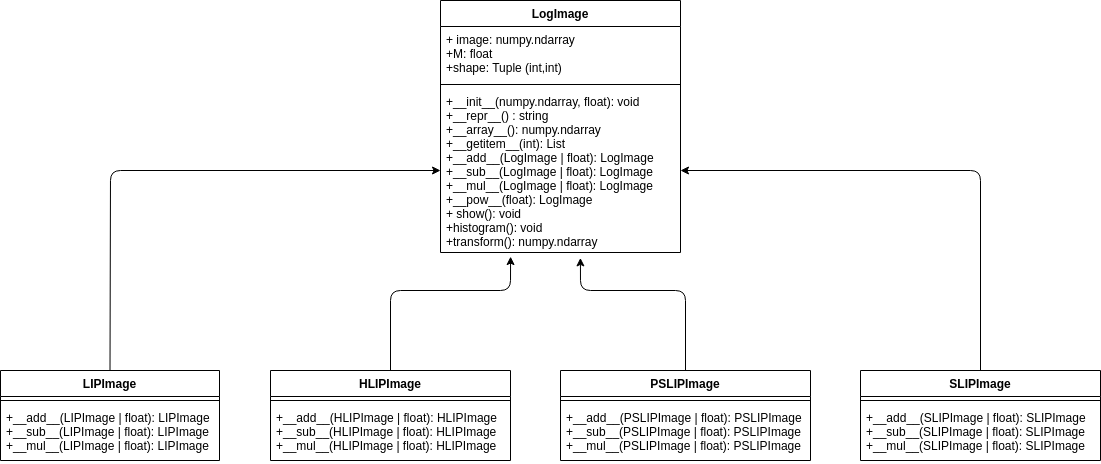
\includegraphics[width=11.0 cm]{images/structures_class_diagram.png}
				\caption{Diagrama de clases de las estructuras no lineales.}
			\end{center}
		\end{figure}
		
	\end{frame}	

	\begin{frame}
		\frametitle{Propuesta -- M\'odulo Implementado -- Espacios}
		
		\begin{figure}
			\begin{center}
				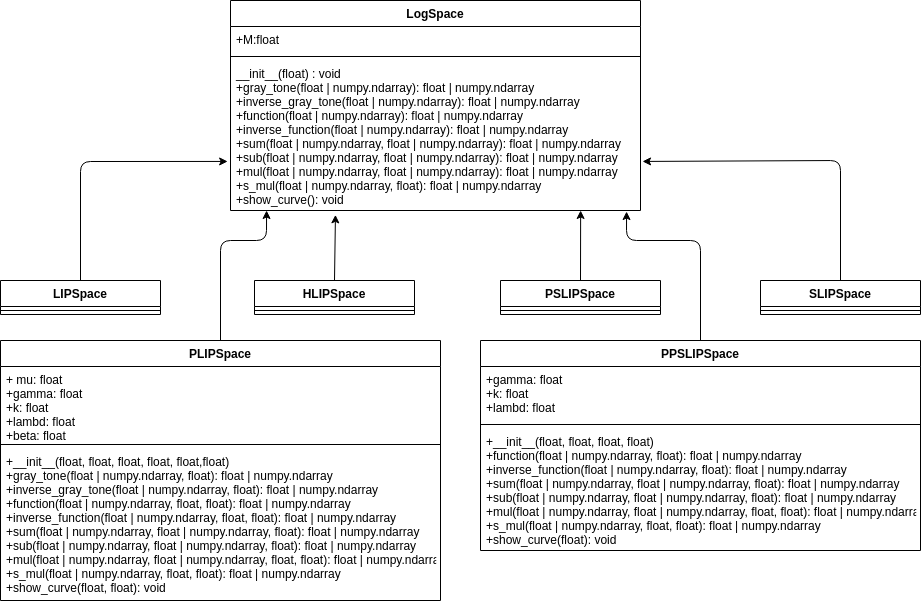
\includegraphics[width=11.0 cm]{images/spaces_class_diagram.png}
				\caption{Diagrama de clases de los espacios no lineales.}
			\end{center}
		\end{figure}
		
	\end{frame}	

	\begin{frame}
		\frametitle{Propuesta -- M\'odulo Implementado -- M\'etricas -- EMEE}
		
		La Medida de Mejora por Entrop�a se calcula dividiendo una imagen $I$ en $k_1 \times k_2$ bloques, obteniendo el m�ximo local $I_{max k,l}$ y el m�nimo $I_{min k,l}$ dentro de cada bloque individualmente, y luego proces�ndolos usando la siguiente ecuaci�n:
		\begin{equation}
			\displaystyle EMEE_{\alpha,k_1,k_2=\frac{1}{k_1k_2}}\sum_{l=1}^{k_1}\sum_{k=1}^{k_2}\alpha\left(\frac{I_{max k,l}}{I_{min k,l}}\right)^\alpha\ln\left(\frac{I_{max k,l}}{I_{min k,l}}\right),
		\end{equation}
		donde $\alpha$ es una constante que puede ayudar a seleccionar los par�metros. Se eligi\'o $\alpha = 1$ y el tama�o de bloque $4 \times 4$, $4 \times 5$, $5 \times 4$ y $5 \times 5$, seg\'un las dimensiones de la imagen.
	\end{frame}
	
	\begin{frame}
		\frametitle{Propuesta -- M\'odulo Implementado -- M\'etricas -- EMEE}
	
		El mejor par�metro (�ptimo) se obtiene si se cumple la siguiente condici�n:
		\begin{equation}
			EMEE_{optimal}=max_{local}(EMEE(\alpha, \mu, \gamma, k, \lambda, \beta))
		\end{equation}
		
		Esta medida se utiliz\'o para obtener las mejores combinaciones de par\'ametros en el modelo PLIP.
		
	\end{frame}

	\begin{frame}
		\frametitle{Propuesta -- M\'odulo Implementado -- M\'etricas -- $C_p$}
		
		El contraste absoluto entre dos p�xeles distintos $p_1, p_2 \in D, D\subseteq\mathbb{R}^2$, para una imagen, $f\in I(D,E)$ se define:
		\begin{equation}
			C_A(p_1,p_2)=\frac{1}{d(p_1,p_2)}\cdot\frac{|f(p_1)-f(p_2)|}{1-\frac{f(p_1)\cdot f(p_2)}{M^2}},
		\end{equation}
	
		Luego de experimentos, se decidi\'o modificar la ecuaci\'on anterior, cambiando la definici\'on a:
		\begin{equation}
			C_A(p_1,p_2)=\frac{|f(p_1)-f(p_2)|}{d(p_1,p_2)}\cdot\frac{256}{M}
		\end{equation}
	\end{frame}
	
	\begin{frame}
		\frametitle{Propuesta -- M\'odulo Implementado -- M\'etricas -- $C_p$}
		
		El contraste para un p�xel arbitrario $p \in D$, para una imagen $f \in I ( D , E )$, se define por la media del contraste absoluto entre el p�xel $p$ y los p�xeles $( p_i )_{i = 1,\cdots,n}$ que pertenecen a una vecindad $V$:
		\begin{equation}
			\displaystyle C(p)=\frac{1}{n}\sum_{i=1}^{n}C_A(p,p_i).
		\end{equation}
	
		Luego el valor de $C_p$ de una imagen es el promedio de los valores de $C(p)$ de los pixeles que la conforman.
		
	\end{frame}	

	\begin{frame}
		\frametitle{Propuesta -- M\'odulo Implementado -- Algoritmos}
		
		\begin{block}{Detecci\'on de bordes}
			Se utilizan diferentes filtros como Sobel, Prewitt, Scharr, etc. En particular los tres mencionados anteriormente aparecen implementados en la librer\'ia \texttt{skimage.filters} de Python.
		\end{block}
	
		\begin{block}{Unsharp masking}
			\textit{Unsharp Masking} es una t\'ecnica para mejorar la calidad de una imagen. Esta t\'ecnica consiste en determinar los bordes de una imagen y luego fusionar la imagen original con la imagen de bordes de dicha imagen.
		\end{block}
	\end{frame}

	\begin{frame}
		\frametitle{Propuesta -- M\'odulo Implementado -- Algoritmos}
		\begin{block}{Transformaci\'on Af\'in}
			Transformaci\'on af\'in  $\psi : I (D, E) \to I (D, E ): E=(a,b)$, para una imagen $f\in I(D,E)$:
			
			\begin{equation}
				\psi(f)=\frac{\sigma_u}{\sigma_f}\otimes(f\ominus\mu_f).
			\end{equation}
			tal que $\mu_f$ es la media de la imagen, $\sigma_f^2$ es la varianza de la imagen y $\sigma_u^2=\frac{(b-a)^2}{12}$.
			
			Importante: Este algoritmo solo se puede utilizar en espacios vectoriales acotados.
			
		\end{block}
	\end{frame}

	\begin{frame}
		\frametitle{Detalles de Implementaci\'on -- Estructura del M\'odulo}
		\begin{figure}
			\begin{center}
				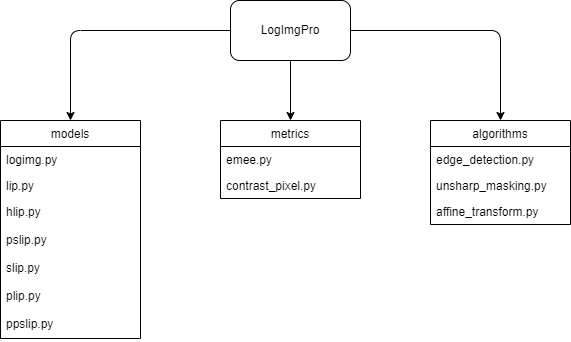
\includegraphics[width=11.0 cm]{images/module_structure.png}
				\caption{Diagrama de la estructura del m\'odulo.}
			\end{center}
		\end{figure}
	\end{frame}


	\begin{frame}
		\frametitle{Experimentos -- Curvas de los Modelos no Parametrizados}
		
		\begin{figure}
			\begin{center}
				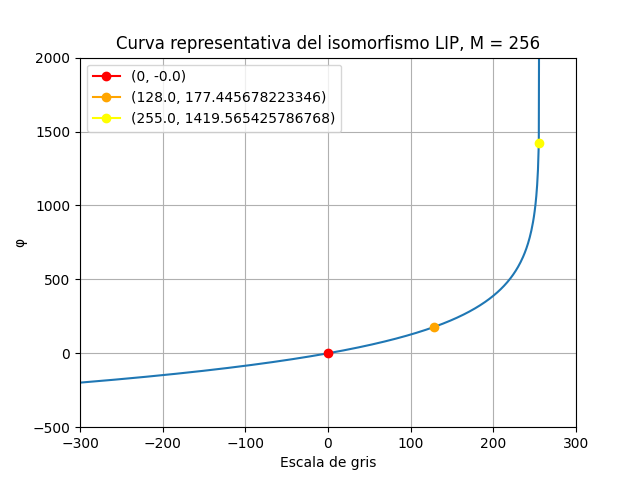
\includegraphics[width=5.0 cm]{images/clasics_curves/lip_curve.png}
				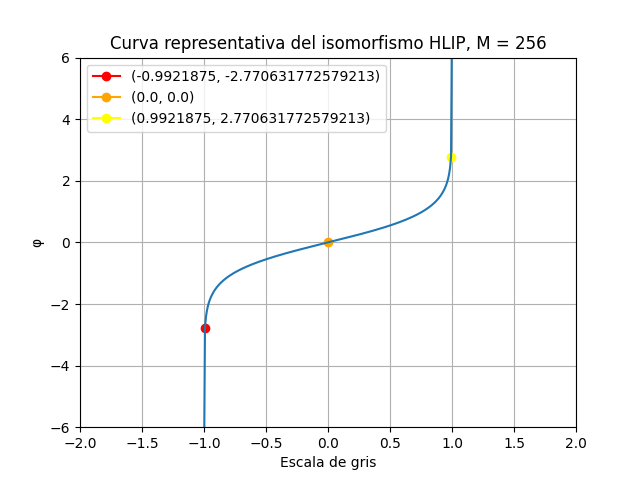
\includegraphics[width=5.0 cm]{images/clasics_curves/hlip_curve.png}
				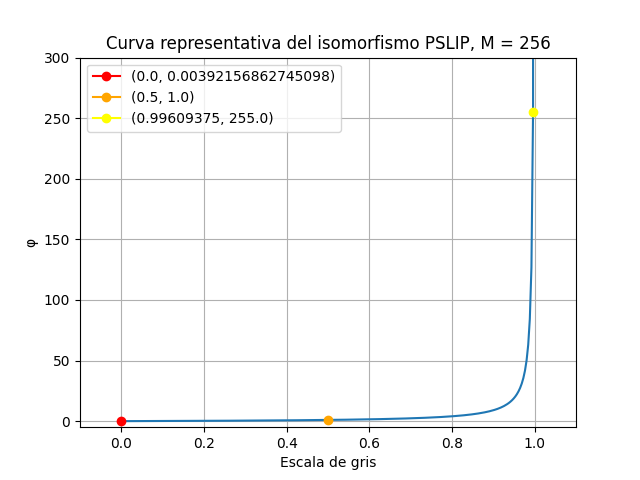
\includegraphics[width=5.0 cm]{images/clasics_curves/pslip_curve.png}
				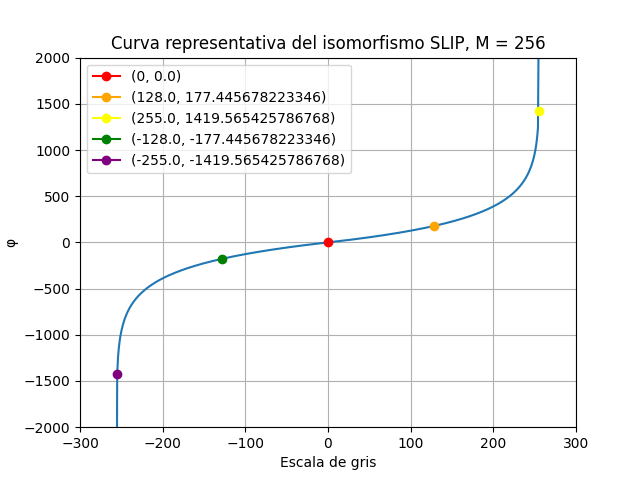
\includegraphics[width=5.0 cm]{images/clasics_curves/slip_curve.png}
				\caption{Curvas representativas de los modelos no parametrizados.}
			\end{center}
		\end{figure}
	\end{frame}

	\begin{frame}
		\frametitle{Experimentos -- Curvas del Modelo PLIP}
		\begin{figure}
			\begin{center}
				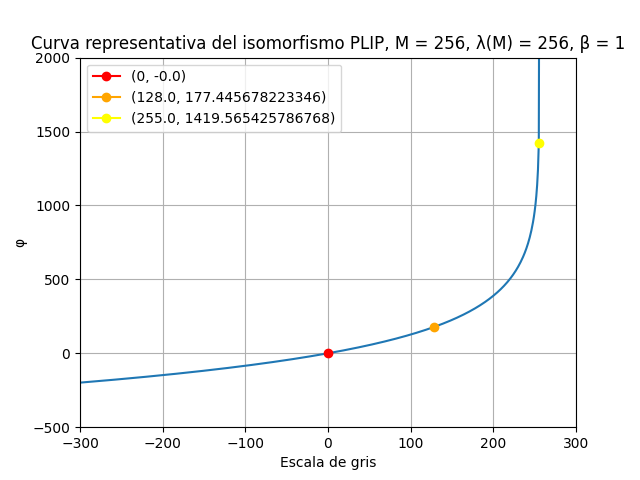
\includegraphics[width=5.0 cm]{images/plip_curves/plip_curve_256.png}
				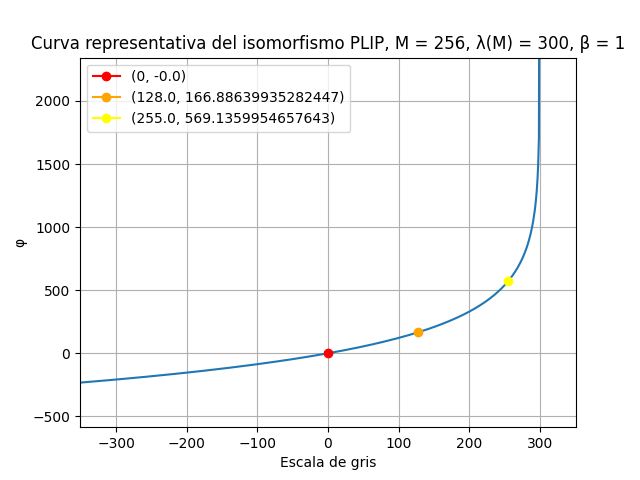
\includegraphics[width=5.0 cm]{images/plip_curves/plip_curve_300.png}
				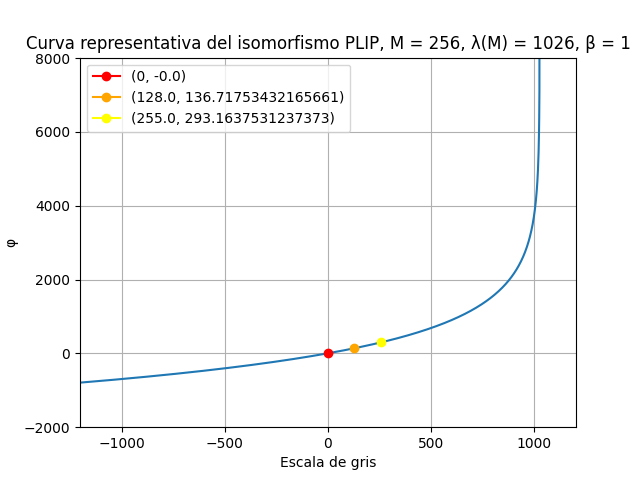
\includegraphics[width=5.0 cm]{images/plip_curves/plip_curve_1026.png}
				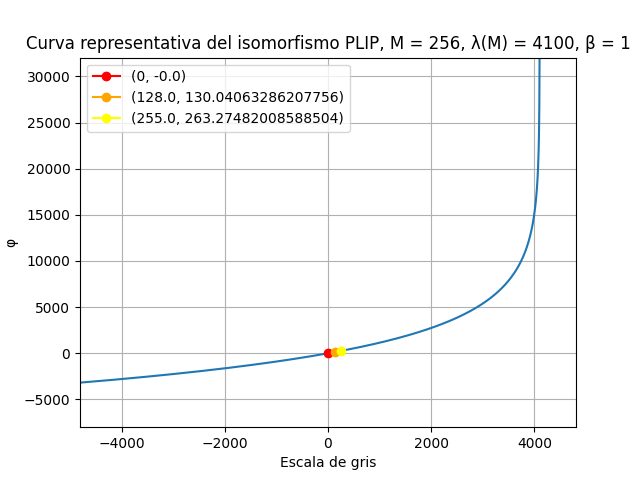
\includegraphics[width=5.0 cm]{images/plip_curves/plip_curve_4100.png}
				\caption{Curvas representativas del modelo PLIP con diferentes valores de $\lambda(M)$.}
			\end{center}
		\end{figure}
	\end{frame}

	\begin{frame}
		\frametitle{Experimentos -- Curvas del Modelo PPSLIP}
		\begin{figure}
			\begin{center}
				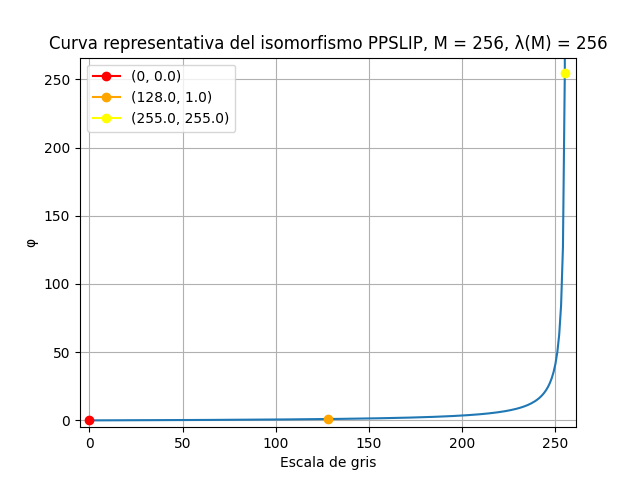
\includegraphics[width=5.0 cm]{images/ppslip_curves/ppslip_curve_256.png}
				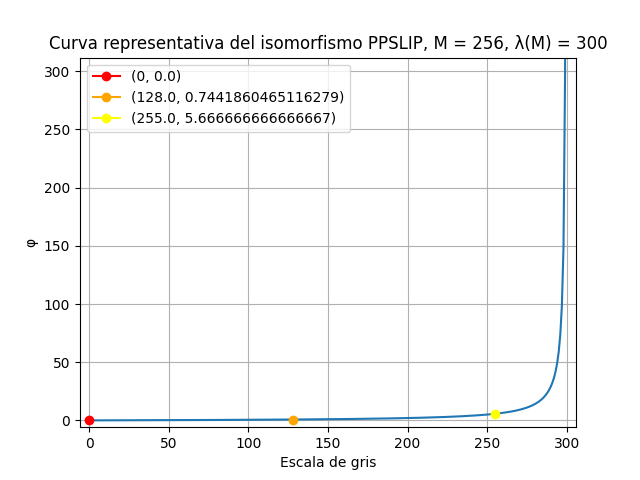
\includegraphics[width=5.0 cm]{images/ppslip_curves/ppslip_curve_300.png}
				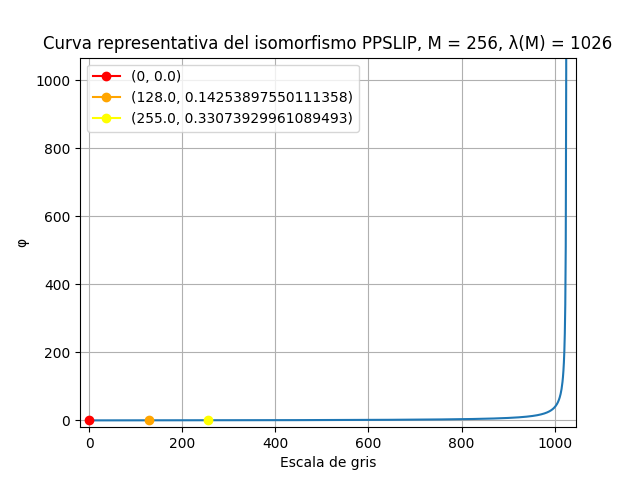
\includegraphics[width=5.0 cm]{images/ppslip_curves/ppslip_curve_1026.png}
				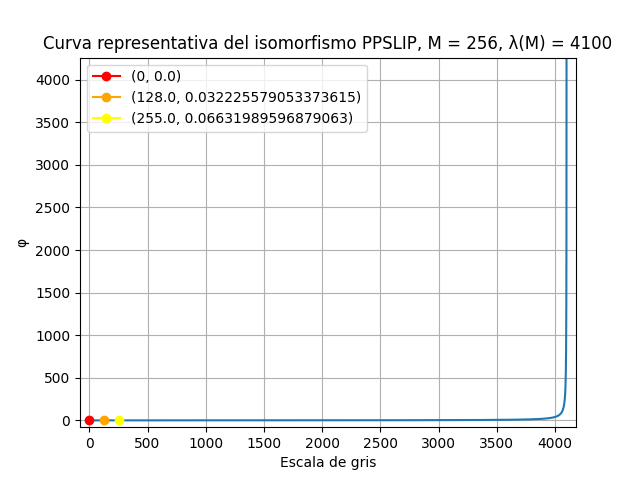
\includegraphics[width=5.0 cm]{images/ppslip_curves/ppslip_curve_4100.png}
				\caption{Curvas representativas del modelo PPSLIP, diferentes valores de $\lambda(M)$.}
			\end{center}
		\end{figure}
	\end{frame}

	\begin{frame}
		\frametitle{Experimentos -- Suma de Im\'agenes}
		
		\begin{figure}[h]
			\begin{center}
				\subfigure[Playa]{
					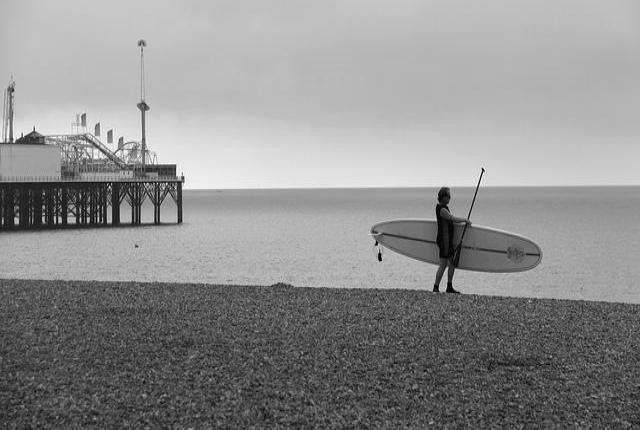
\includegraphics[width=4.5 cm]{images/originals/playa.jpg}}
				\subfigure[Patineta]{
					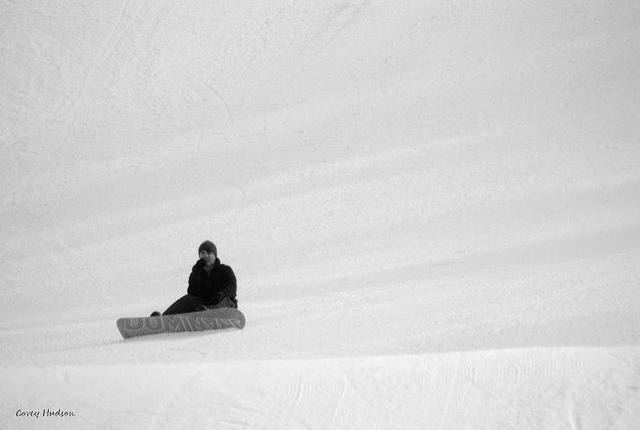
\includegraphics[width=4.5 cm]{images/originals/patineta.jpg}}
				\subfigure[Monta\~na]{
					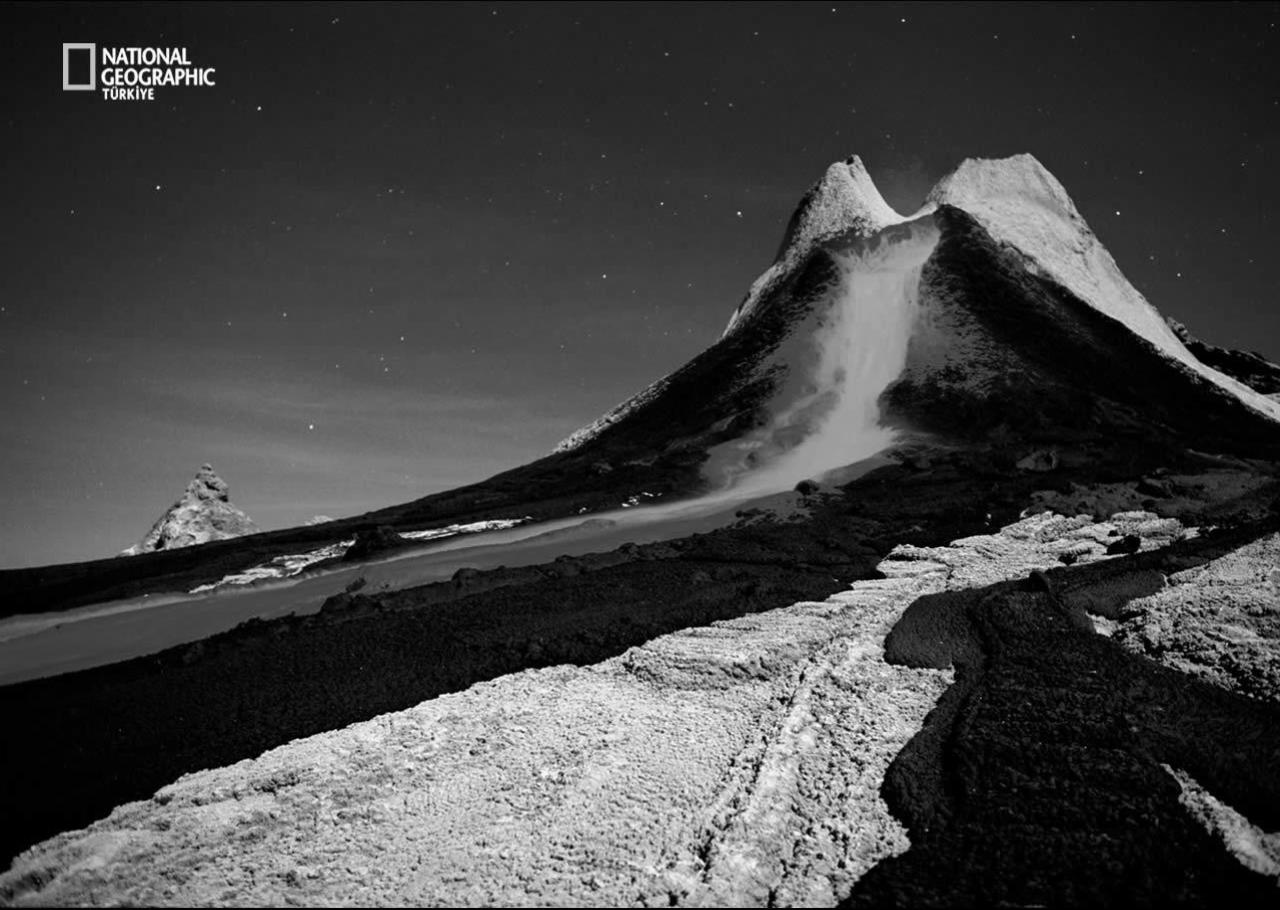
\includegraphics[width=4.5 cm]{images/originals/montania.jpg}}
				\subfigure[Insecto]{
					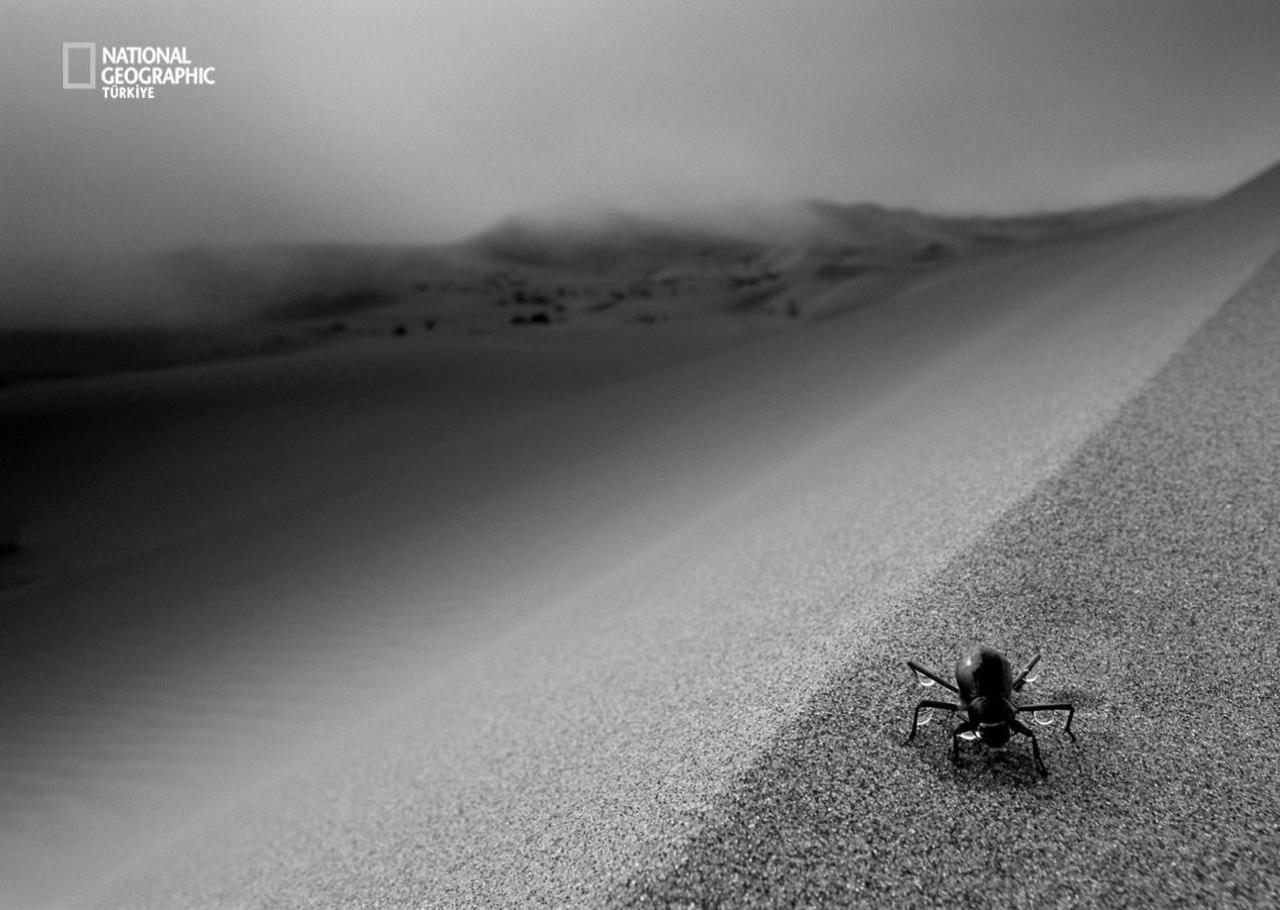
\includegraphics[width=4.5 cm]{images/originals/insecto.jpg}}
				\caption{Im\'agenes para los experimentos de suma.}
			\end{center}
		\end{figure}
		
	\end{frame}

	\begin{frame}
		\frametitle{Experimentos -- Suma de Im\'agenes -- Playa y Patineta}
		\begin{figure}
			\begin{center}
				\subfigure[Lineal $C_p=3.49$]{
					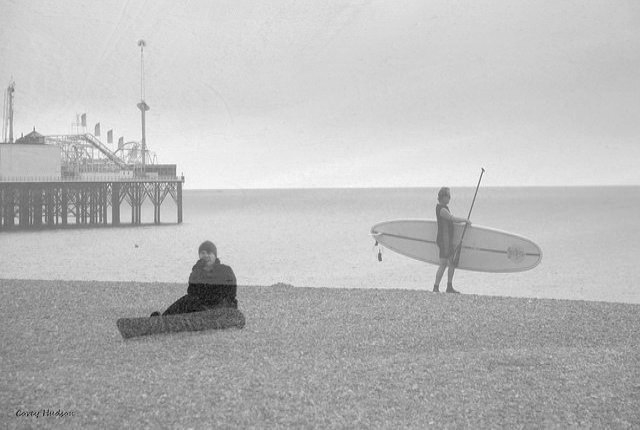
\includegraphics[width=3.0 cm]{images/sums/p y p/sab.png}}
				\subfigure[LIP $C_p=5.71$]{
					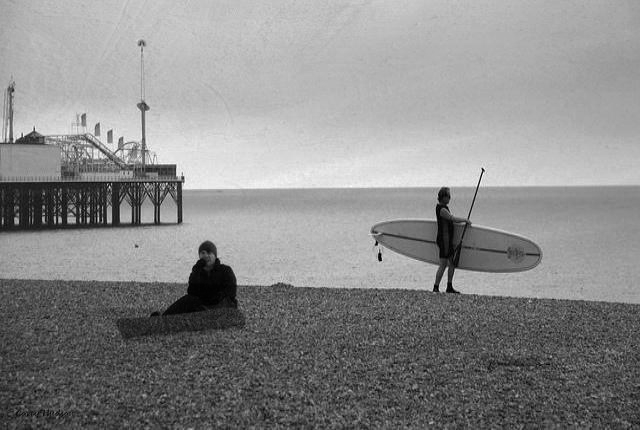
\includegraphics[width=3.0 cm]{images/sums/p y p/jsab.png}}
				\subfigure[HLIP $C_p=4.96$]{
					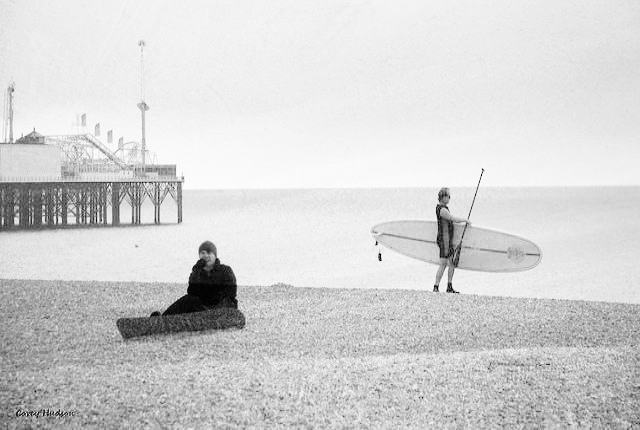
\includegraphics[width=3.0 cm]{images/sums/p y p/hsab.png}}
				\subfigure[PSLIP $C_p=1.39$]{
					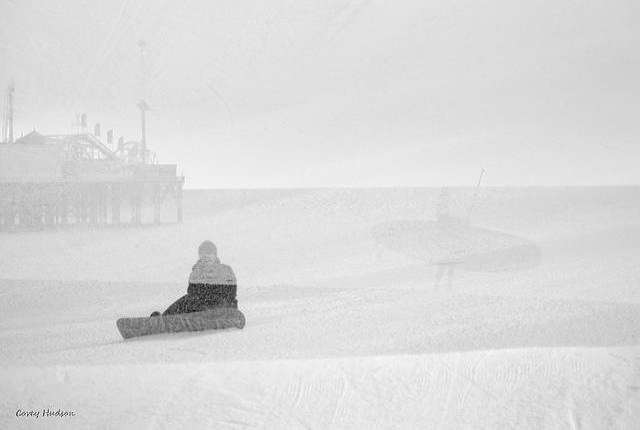
\includegraphics[width=3.0 cm]{images/sums/p y p/pssab.png}}
				\subfigure[SLIP $C_p=1.45$]{
					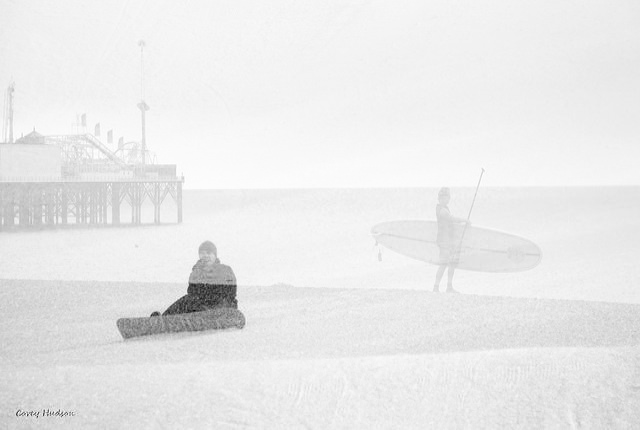
\includegraphics[width=3.0 cm]{images/sums/p y p/ssab.png}}
				\subfigure[PLIP $C_p=5.71$]{
					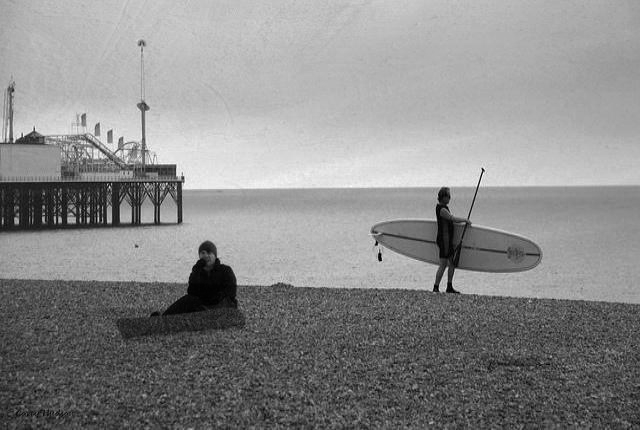
\includegraphics[width=3.0 cm]{images/sums/p y p/psab.png}}
				\subfigure[PPSLIP $C_p=3.35$]{
					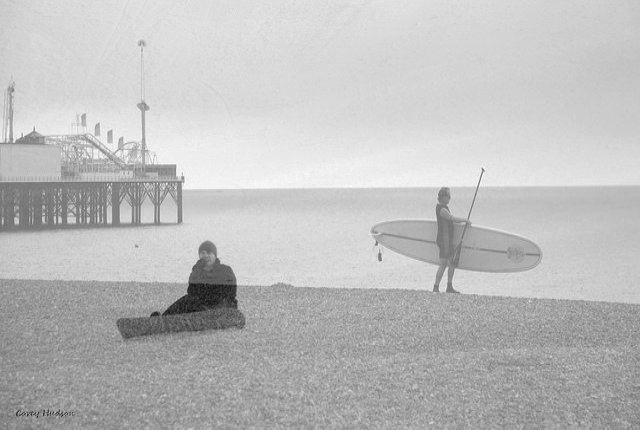
\includegraphics[width=3.0 cm]{images/sums/p y p/ppssab.png}}
			\end{center}
		\end{figure}
	\end{frame}

	\begin{frame}
		\frametitle{Experimentos -- Suma de Im\'agenes -- Monta\~na e Insecto}
		\begin{figure}
			\begin{center}
				\subfigure[Lineal $C_p=3.15$]{
					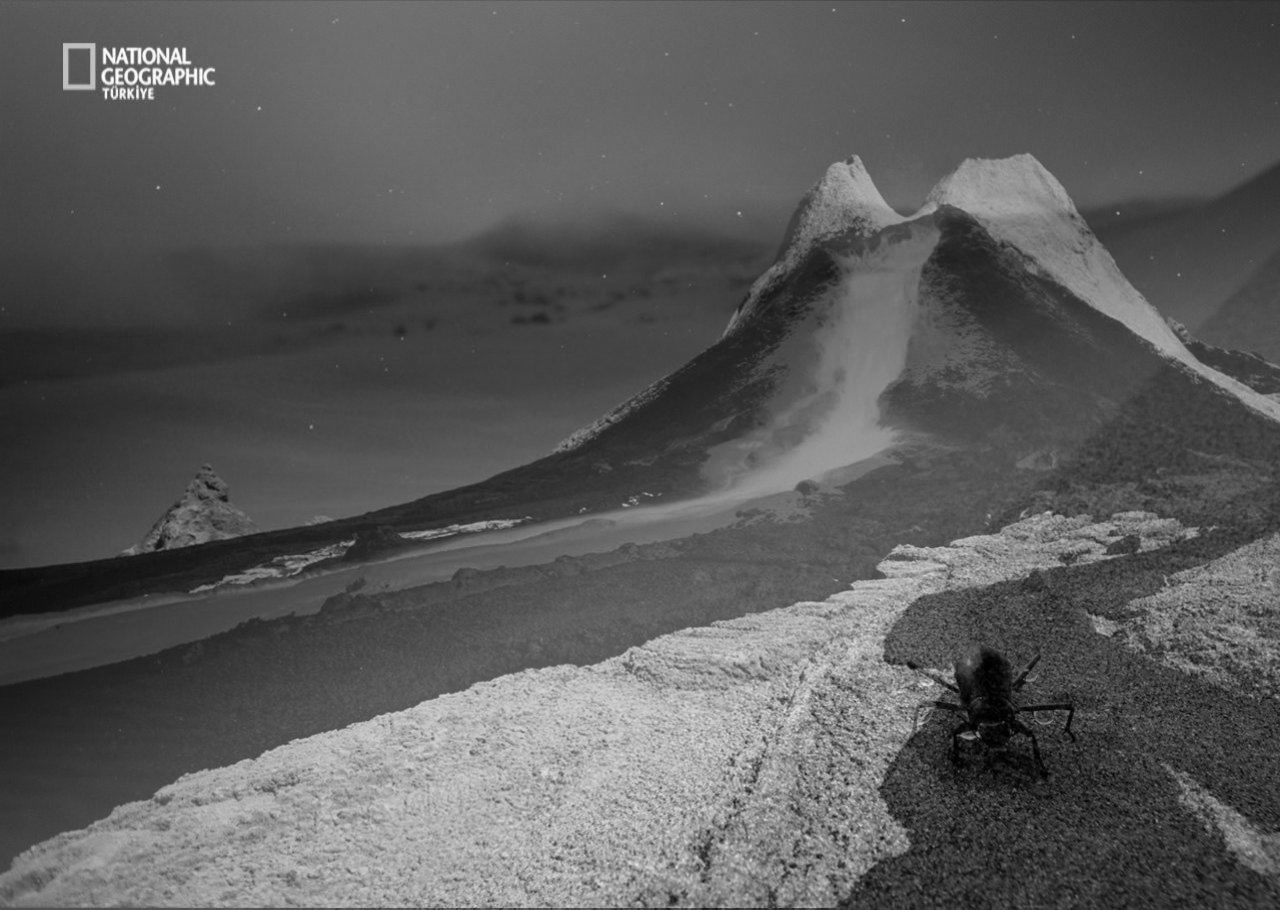
\includegraphics[width=2.8 cm]{images/sums/m y i/scd.png}}
				\subfigure[LIP $C_p=2.77$]{
					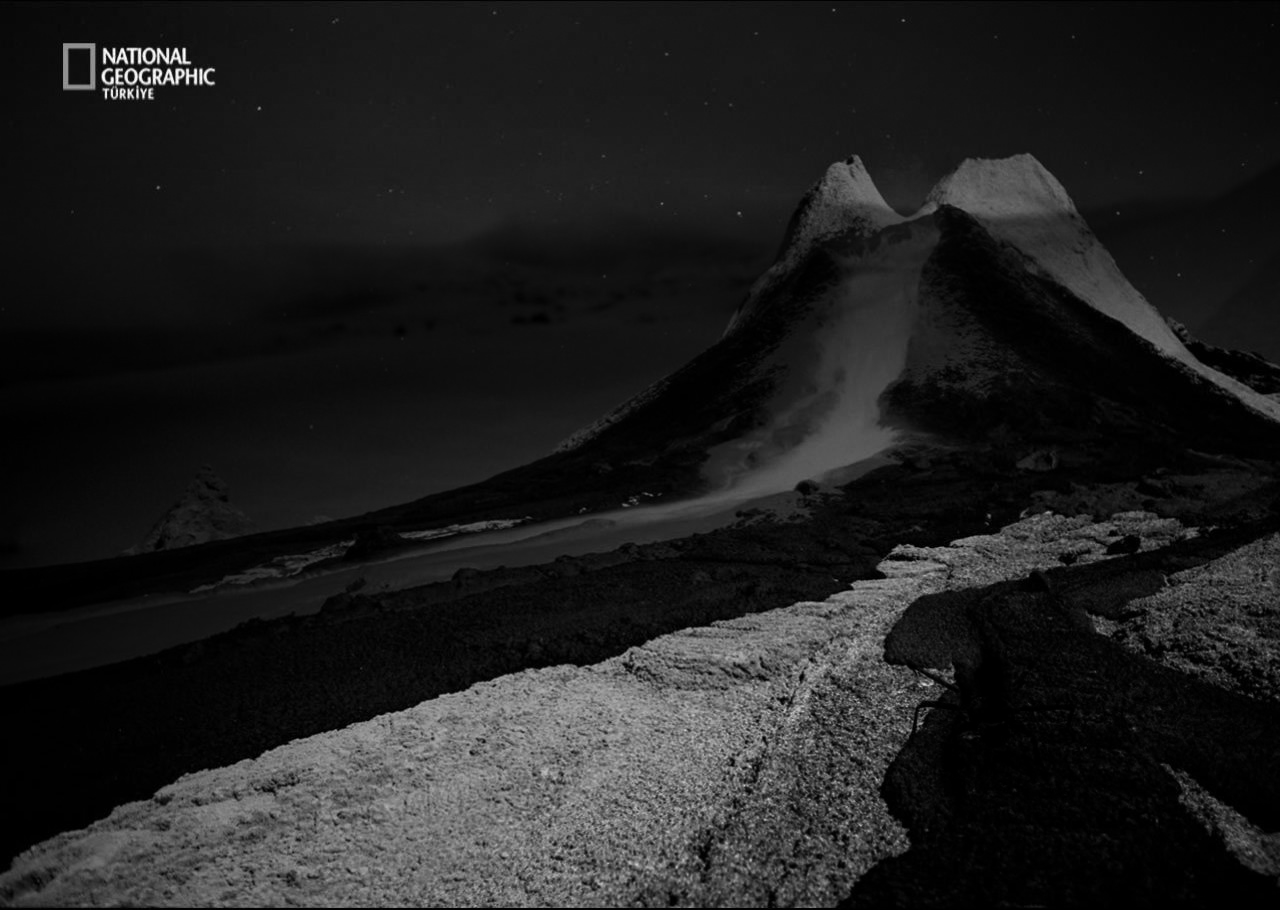
\includegraphics[width=2.8 cm]{images/sums/m y i/jscd.png}}
				\subfigure[HLIP $C_p=4.53$]{
					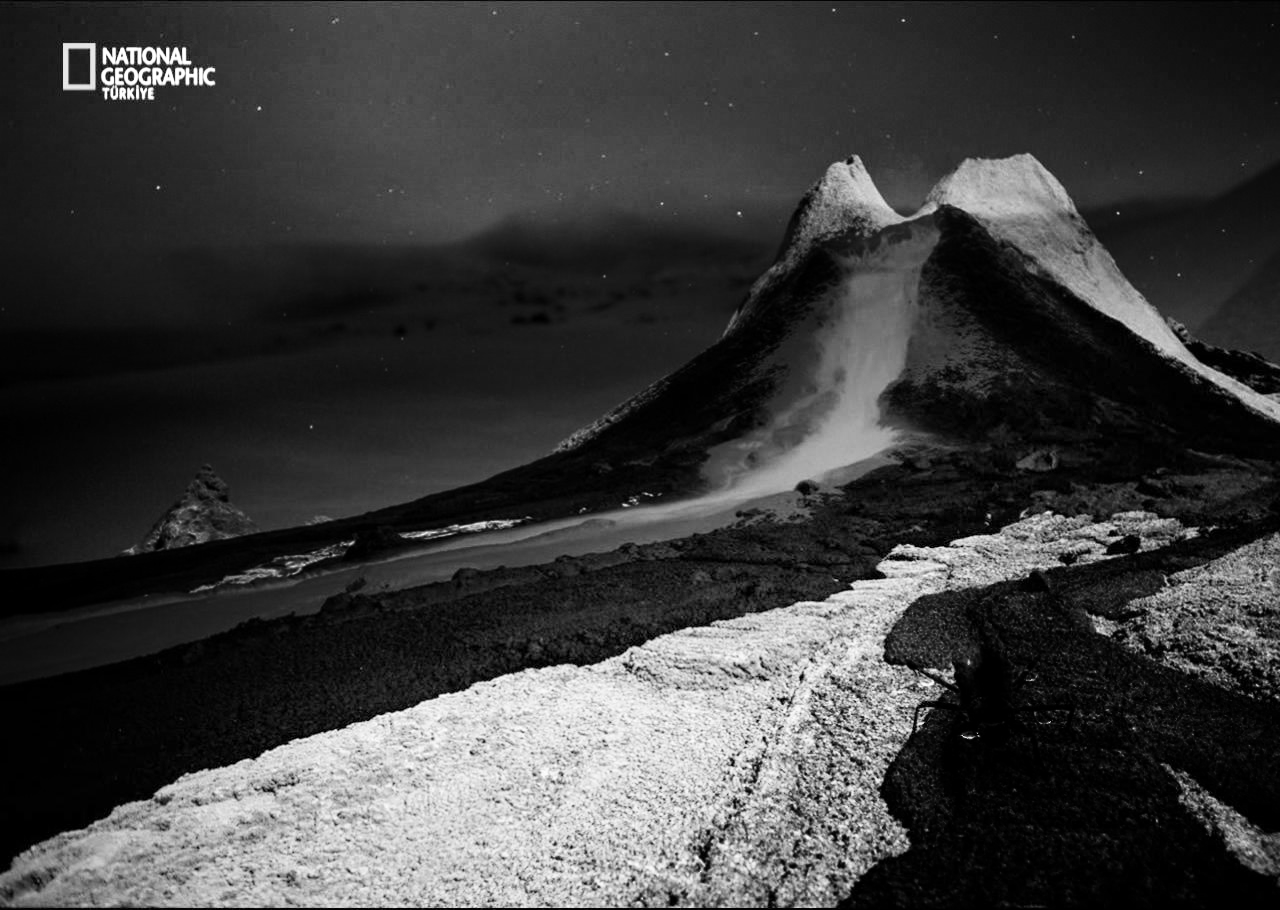
\includegraphics[width=2.8 cm]{images/sums/m y i/hscd.png}}
				\subfigure[PSLIP $C_p=3.47$]{
					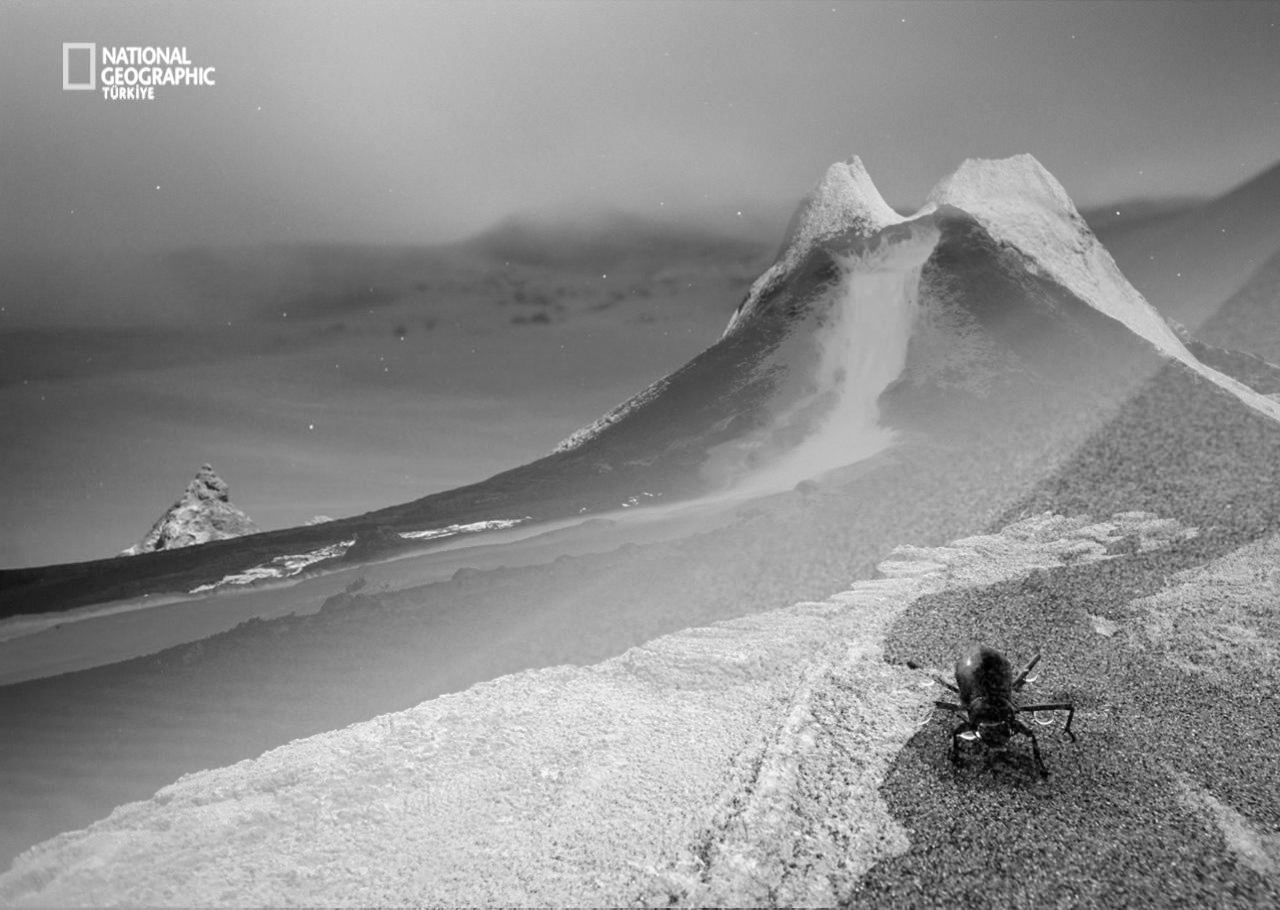
\includegraphics[width=2.8 cm]{images/sums/m y i/psscd.png}}
				\subfigure[SLIP $C_p=3.65$]{
					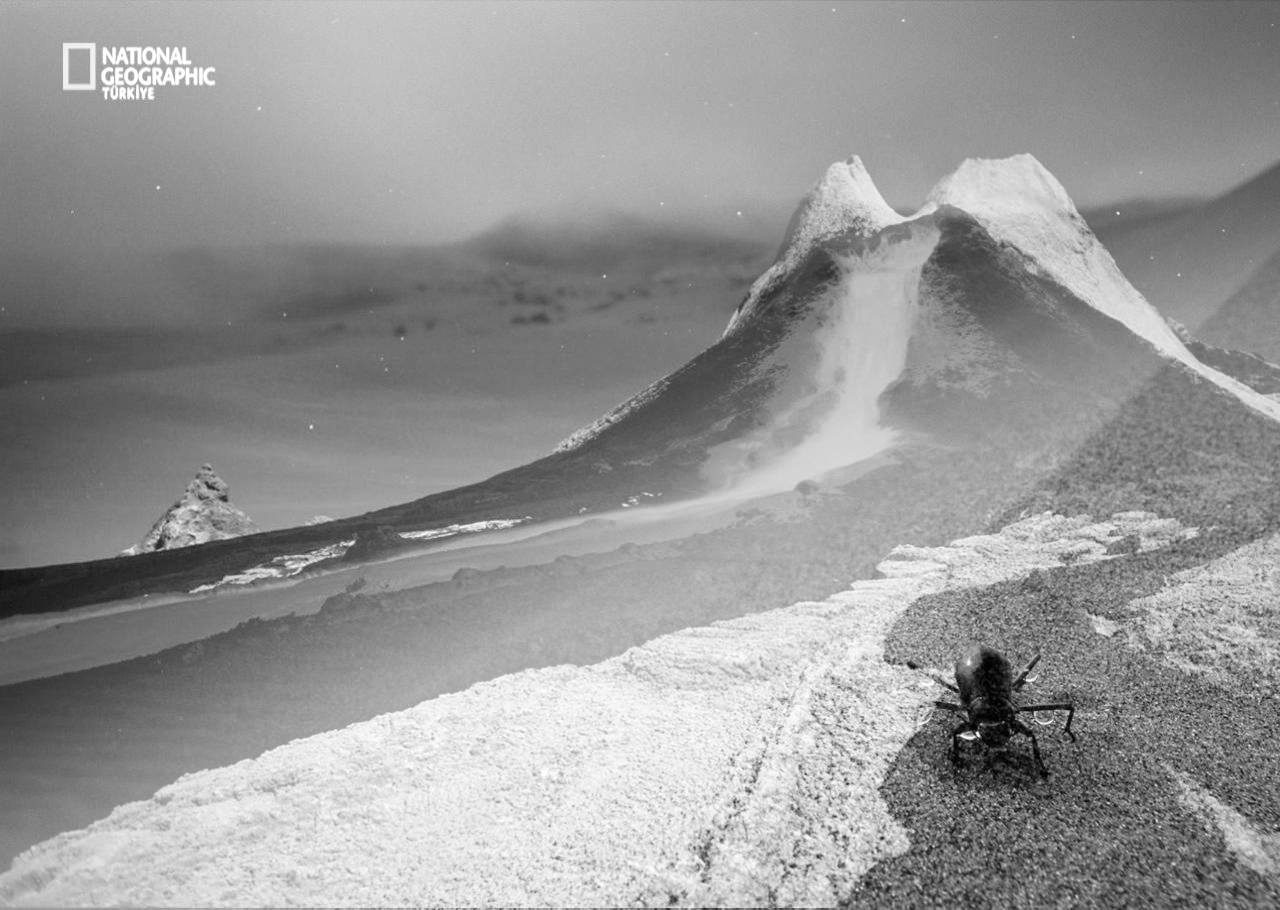
\includegraphics[width=2.8 cm]{images/sums/m y i/sscd.png}}
				\subfigure[PLIP $C_p=3.13$]{
					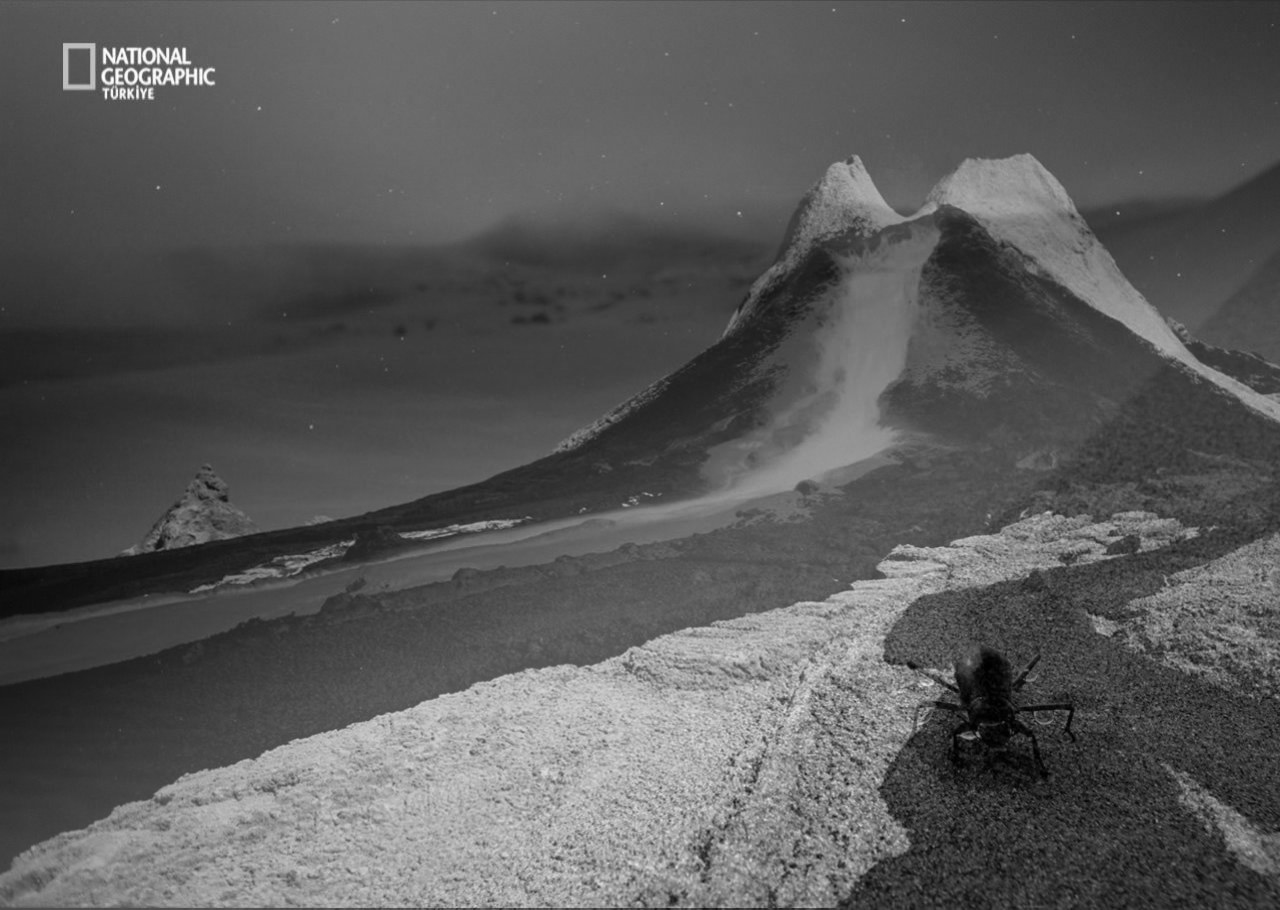
\includegraphics[width=2.8 cm]{images/sums/m y i/pscd.png}}
				\subfigure[PPSLIP $C_p=3.47$]{
					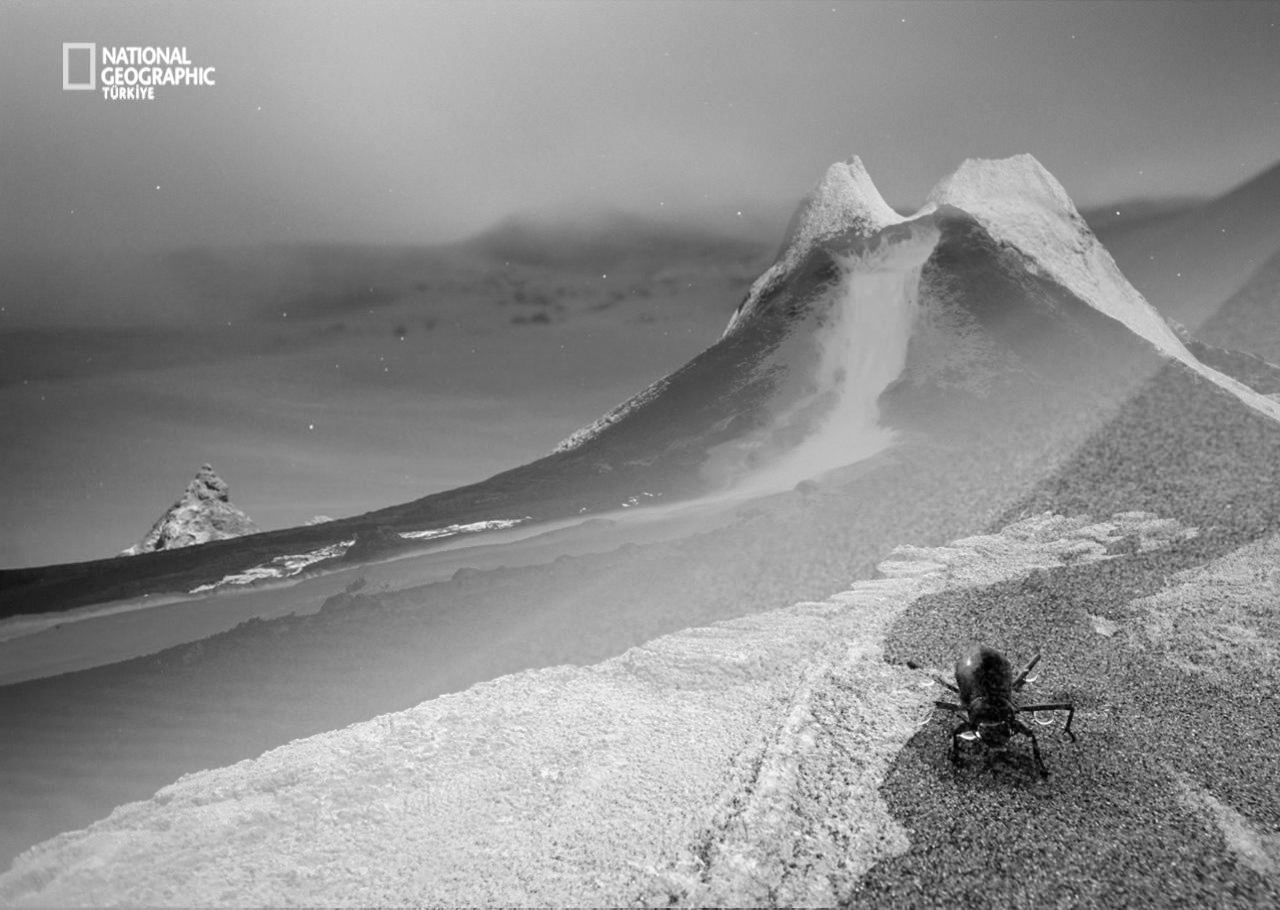
\includegraphics[width=2.8 cm]{images/sums/m y i/ppsscd.png}}
				\caption{Suma de Monta\~na e Insecto utilizando los diferentes modelos.}
			\end{center}
		\end{figure}
	\end{frame}

	\begin{frame}
		\frametitle{Experimentos -- Suma de Im\'agenes -- Estad\'isticas}
		\begin{figure}
			\begin{center}
				\subfigure[Diagramas de caja para la medida $C_p$.]{
				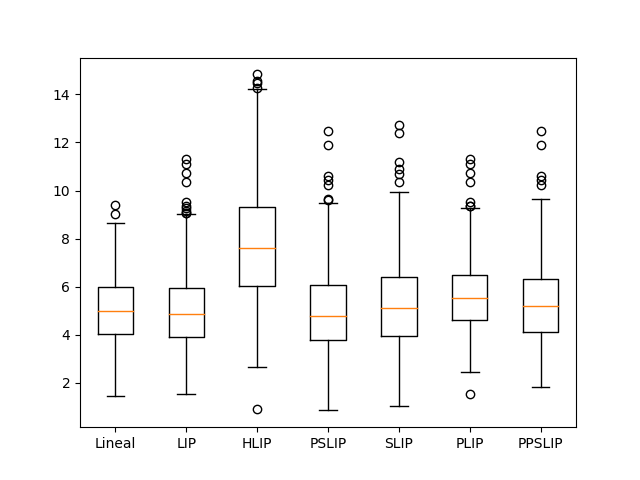
\includegraphics[width=6.0 cm]{images/graphics/sum_all.png}}
				\subfigure[Media y mediana del valor de $C_p$.]{
				\resizebox{4.0 cm}{1.5 cm}{
				\begin{tabular}{|l|l|l|}
					\hline 
					Modelo & Media & Mediana\\
					\hline
					Lineal & $5.05$ & $4.98$\\
					\hline
					LIP & $5.00$ & $4.85$\\
					\hline
					HLIP & $7.73$ & $7.59$\\
					\hline
					PSLIP & $4.95$ & $4.78$\\
					\hline
					SLIP & $5.24$ & $5.08$\\
					\hline
					PLIP & $5.60$ & $5.54$\\
					\hline
					PPSLIP & $5.35$ & $5.20$\\
					\hline
				\end{tabular}}}
			\caption{An\'alisis estad\'istico de la operaci\'on suma de los diferentes modelos utilizando im\'agenes naturales.}	
			\end{center}
		\end{figure}
	\end{frame}
	
	\begin{frame}
		\frametitle{Experimentos -- Im\'agenes Utilizadas}
		
		\begin{figure}[h]
			\begin{center}
				\subfigure[C\'amara $C_p=5.00$]{
					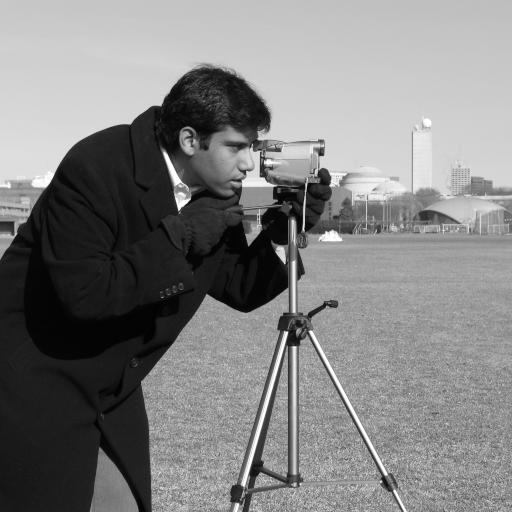
\includegraphics[width=5.0 cm]{images/originals/camera.jpg}}
				\subfigure[T\'orax 1 $C_p=2.26$]{
					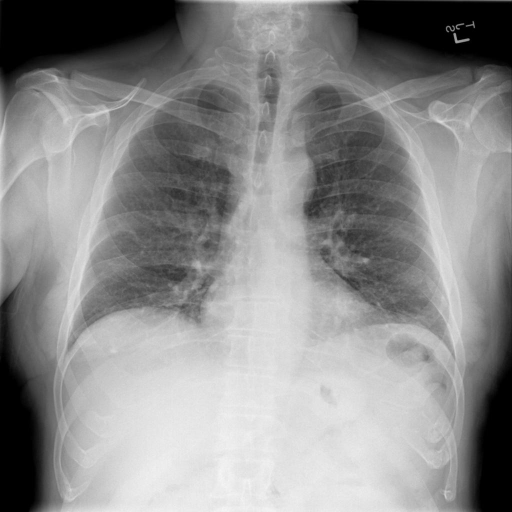
\includegraphics[width=5.0 cm]{images/originals/torax.png}}
				\caption{Im\'agenes para los experimentos de detecci\'on de bordes.}
			\end{center}
		\end{figure}
	\end{frame}

	\begin{frame}
		\frametitle{Experimentos -- Detecci\'on de Bordes -- C\'amara}
		\begin{figure}
			\begin{center}
				\subfigure[Lineal $C_p=4.69$]{
					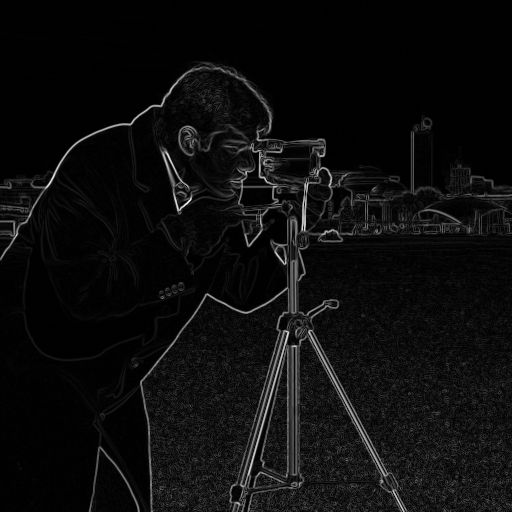
\includegraphics[width=2.5 cm]{images/scharr/camera/sla.png}}
				\subfigure[LIP $C_p=7.43$]{
					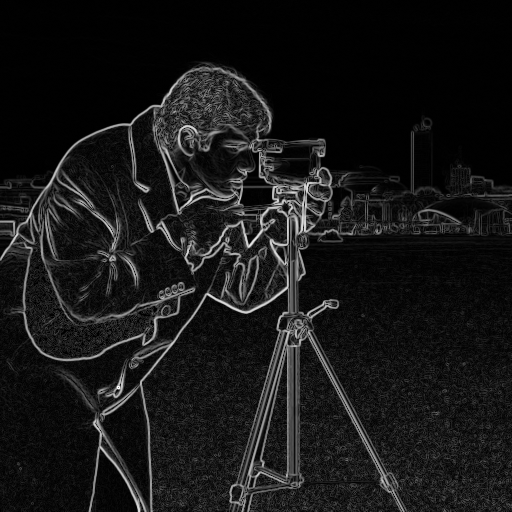
\includegraphics[width=2.5 cm]{images/scharr/camera/sja.png}}
				\subfigure[HLIP $C_p=8.05$]{
					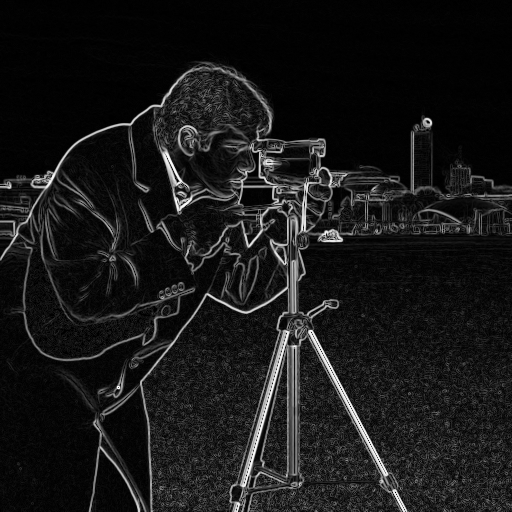
\includegraphics[width=2.5 cm]{images/scharr/camera/sha.png}}
				\subfigure[PSLIP $C_p=9.41$]{
					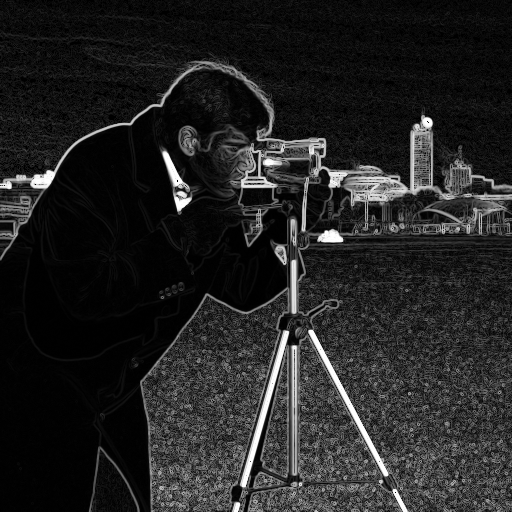
\includegraphics[width=2.5 cm]{images/scharr/camera/spsa.png}}
				\subfigure[SLIP $C_p=6.26$]{
					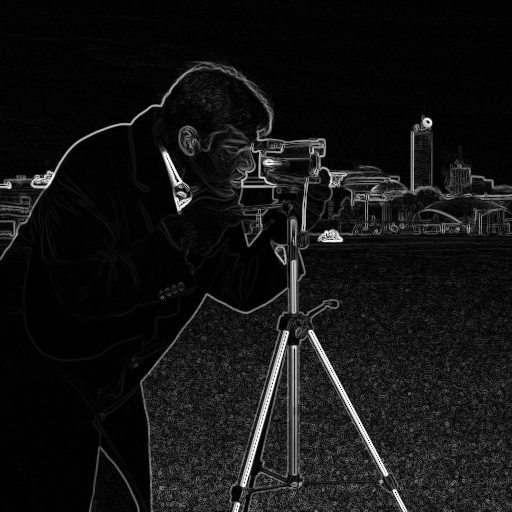
\includegraphics[width=2.5 cm]{images/scharr/camera/ssa.png}}
				\subfigure[PLIP $C_p=7.43$]{
					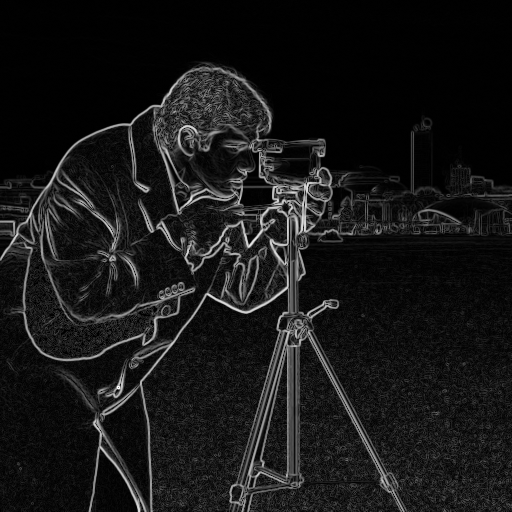
\includegraphics[width=2.5 cm]{images/scharr/camera/spa.png}}
				\subfigure[PPSLIP $C_p=9.41$]{
					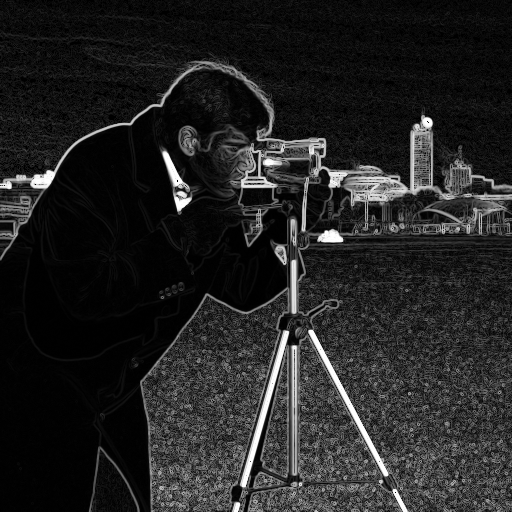
\includegraphics[width=2.5 cm]{images/scharr/camera/sppsa.png}}
				\caption{Filtro de Scharr aplicado a la imagen C\'amara con los diferentes modelos.}
			\end{center}
		\end{figure}
	\end{frame}

	\begin{frame}
		\frametitle{Experimentos -- Detecci\'on de Bordes -- T\'orax 1}
		\begin{figure}
			\begin{center}
				\subfigure[Lineal $C_p=2.89$]{
					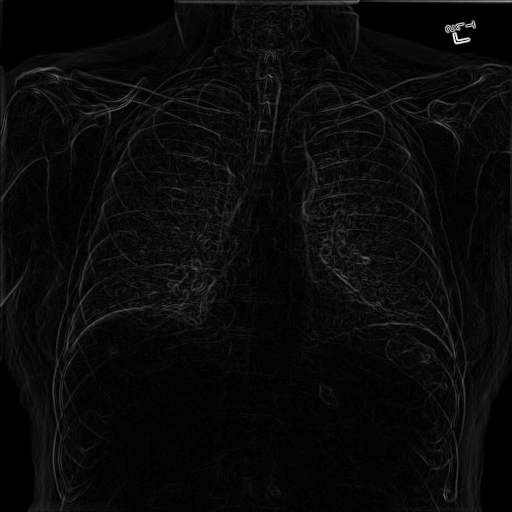
\includegraphics[width=2.5 cm]{images/scharr/torax/slb.png}}
				\subfigure[LIP $C_p=3.66$]{
					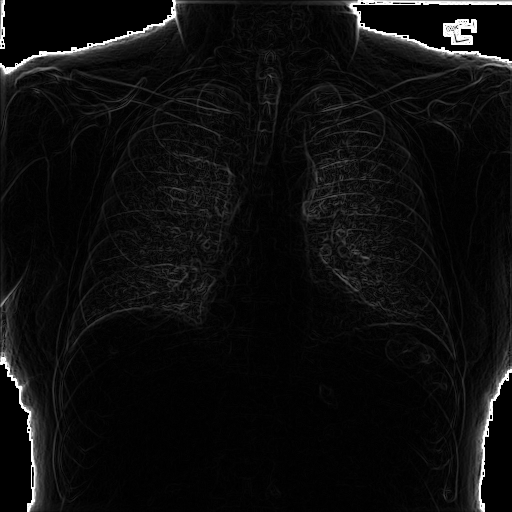
\includegraphics[width=2.5 cm]{images/scharr/torax/sjb.png}}
				\subfigure[HLIP $C_p=4.40$]{
					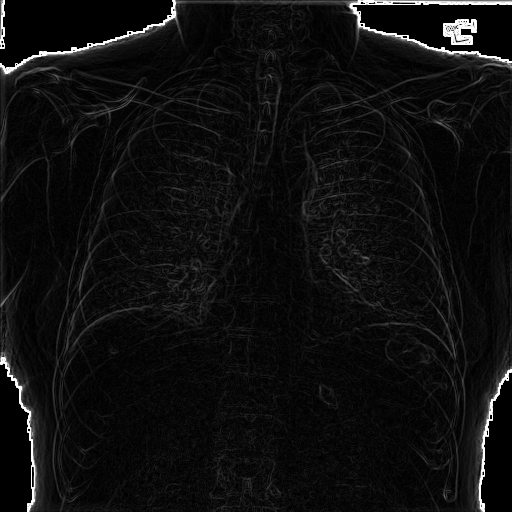
\includegraphics[width=2.5 cm]{images/scharr/torax/shb.png}}
				\subfigure[PSLIP $C_p=9.73$]{
					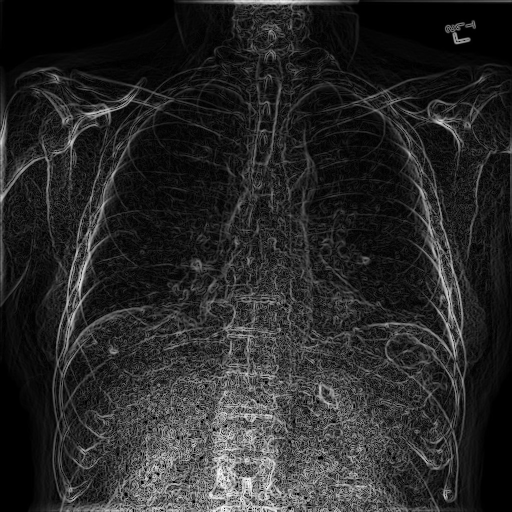
\includegraphics[width=2.5 cm]{images/scharr/torax/spsb.png}}
				\subfigure[SLIP $C_p=6.85$]{
					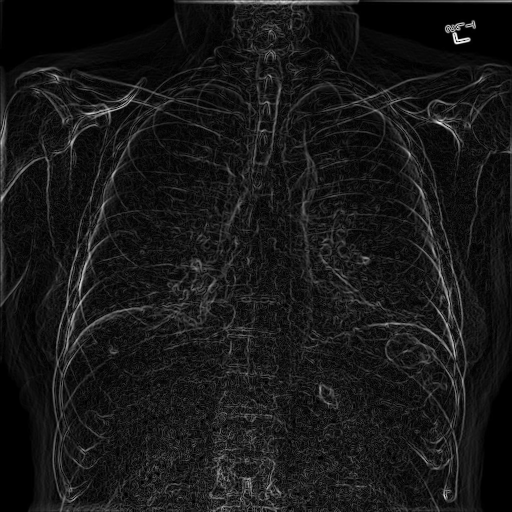
\includegraphics[width=2.5 cm]{images/scharr/torax/ssb.png}}
				\subfigure[PLIP $C_p=3.66$]{
					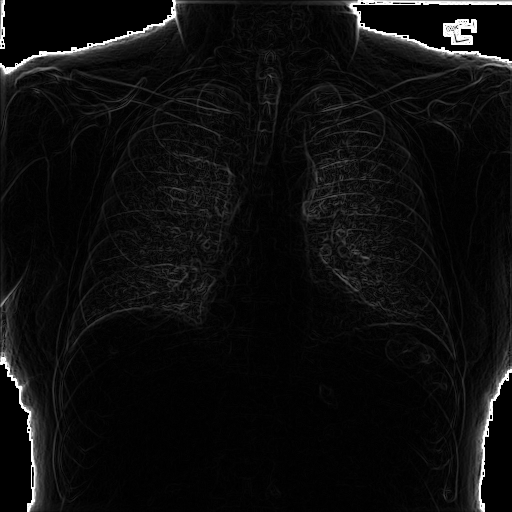
\includegraphics[width=2.5 cm]{images/scharr/torax/spb.png}}
				\subfigure[PPSLIP $C_p=9.73$]{
					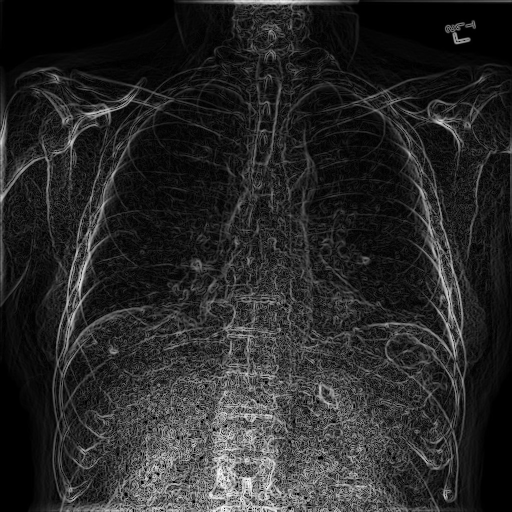
\includegraphics[width=2.5 cm]{images/scharr/torax/sppsb.png}}
				\caption{Filtro de Scharr aplicado a la imagen T\'orax 1 con los diferentes modelos.}
			\end{center}
		\end{figure} 
	\end{frame}
	
	\begin{frame}
		\frametitle{Experimentos -- Detecci\'on de Bordes -- Estad\'isticas}
		\begin{figure}
			\begin{center}
				\subfigure[Diagramas de caja para la medida $C_p$.]{
					\includegraphics[width=6.0 cm]{images/graphics/natural/ed/ed_all.png}}
				\subfigure[Media y mediana del valor de $C_p$.]{
					\resizebox{4.0 cm}{1.7 cm}{
					\begin{tabular}{|l|l|l|}
						\hline 
						Modelo & Media & Mediana\\
						\hline
						Lineal & $5.02$ & $4.75$\\
						\hline
						LIP & $11.55$ & $10.82$\\
						\hline
						HLIP & $12.81$ & $12.36$\\
						\hline
						PSLIP & $11.57$ & $11.38$\\
						\hline
						SLIP & $9.30$ & $8.91$\\
						\hline
						PLIP & $11.59$ & $10.82$\\
						\hline
						PPSLIP & $11.65$ & $11.47$\\
						\hline
					\end{tabular}}}
				\caption{An\'alisis estad\'istico para la medida $C_p$ utilizando los diferentes modelos para la detecci\'on de bordes en im\'agenes naturales.}	
			\end{center}
		\end{figure}
	\end{frame}

	\begin{frame}
		\frametitle{Experimentos -- Detecci\'on de Bordes -- Estad\'isticas}
		\begin{figure}
			\begin{center}
				\subfigure[Diagramas de caja para la medida $C_p$.]{
					\includegraphics[width=6.0 cm]{images/graphics/torax/ed/ed_all.png}}
				\subfigure[Media y mediana del valor de $C_p$.]{
					\resizebox{4.0 cm}{1.7 cm}{
						\begin{tabular}{|l|l|l|}
							\hline 
							Modelo & Media & Mediana\\
							\hline
							Lineal & $0.96$ & $0.89$\\
							\hline
							LIP & $3.48$ & $3.38$\\
							\hline
							HLIP & $3.69$ & $3.85$\\
							\hline
							PSLIP & $5.55$ & $5.38$\\
							\hline
							SLIP & $3.11$ & $3.09$\\
							\hline
							PLIP & $3.68$ & $3.60$\\
							\hline
							PPSLIP & $5.64$ & $5.41$\\
							\hline
						\end{tabular}}}
				\caption{An\'alisis estad\'istico para la medida $C_p$ utilizando los diferentes modelos para la detecci\'on de bordes en im\'agenes de radiograf\'ias de t\'orax.}	
			\end{center}
		\end{figure}
	\end{frame}

	\begin{frame}
		\frametitle{Experimentos -- Unsharp Masking -- C\'amara}
		\begin{figure}
			\begin{center}
				\subfigure[Lineal $C_p=4.13$]{
					\includegraphics[width=2.5 cm]{images/unsharp_masking/camera/la_sla.png}}
				\subfigure[LIP $C_p=5.14$]{
					\includegraphics[width=2.5 cm]{images/unsharp_masking/camera/ja_sja.png}}
				\subfigure[HLIP+ $C_p=5.66$]{
					\includegraphics[width=2.5 cm]{images/unsharp_masking/camera/ha_sha+.png}}
				\subfigure[HLIP- $C_p=5.73$]{
					\includegraphics[width=2.5 cm]{images/unsharp_masking/camera/ha_sha-.png}}
				\subfigure[PSLIP $C_p=4.84$]{
					\includegraphics[width=2.5 cm]{images/unsharp_masking/camera/psa_spsa.png}}
				\subfigure[SLIP $C_p=5.16$]{
					\includegraphics[width=2.5 cm]{images/unsharp_masking/camera/sa_ssa.png}}
				\subfigure[PLIP $C_p=5.14$]{
					\includegraphics[width=2.5 cm]{images/unsharp_masking/camera/pa_spa.png}}
				\subfigure[PPSLIP $C_p=5.80$]{
					\includegraphics[width=2.5 cm]{images/unsharp_masking/camera/ppsa_sppsa.png}}
				\caption{Unsharp masking aplicado a la imagen C\'amara con los diferentes modelos.}
			\end{center}
		\end{figure}
	\end{frame}
	
	\begin{frame}
		\frametitle{Experimentos -- Unsharp Masking -- T\'orax 1}
		\begin{figure}
			\begin{center}
				\subfigure[Lineal $C_p=2.60$]{
					\includegraphics[width=2.5 cm]{images/unsharp_masking/torax/lb_slb.png}}
				\subfigure[LIP $C_p=2.53$]{
					\includegraphics[width=2.5 cm]{images/unsharp_masking/torax/jb_sjb.png}}
				\subfigure[HLIP+ $C_p=3.46$]{
					\includegraphics[width=2.5 cm]{images/unsharp_masking/torax/hb_shb+.png}}
				\subfigure[HLIP- $C_p=2.62$]{
					\includegraphics[width=2.5 cm]{images/unsharp_masking/torax/hb_shb-.png}}
				\subfigure[PSLIP $C_p=2.52$]{
					\includegraphics[width=2.5 cm]{images/unsharp_masking/torax/psb_spsb.png}}
				\subfigure[SLIP $C_p=2.59$]{
					\includegraphics[width=2.5 cm]{images/unsharp_masking/torax/sb_ssb.png}}
				\subfigure[PLIP $C_p=2.53$]{
					\includegraphics[width=2.5 cm]{images/unsharp_masking/torax/pb_spb.png}}
				\subfigure[PPSLIP $C_p=4.97$]{
					\includegraphics[width=2.5 cm]{images/unsharp_masking/torax/ppsb_sppsb.png}}
				\caption{Unsharp masking aplicado a la imagen T\'orax 1 con los diferentes modelos.}
			\end{center}
		\end{figure}
	\end{frame}
	
	\begin{frame}
		\frametitle{Experimentos -- Unsharp Masking -- Estad\'isticas}
		\begin{figure}
			\begin{center}
				\subfigure[Diagramas de caja para la medida $C_p$.]{
					\includegraphics[width=6.0 cm]{images/graphics/natural/unsharp_masking/um_all.png}}
				\subfigure[Media y mediana del valor de $C_p$.]{
					\resizebox{4.0 cm}{2.0 cm}{
						\begin{tabular}{|l|l|l|}
							\hline 
							Modelo & Media & Mediana\\
							\hline
							Original & $7.63$ & $7.07$\\
							\hline
							Lineal & $6.04$ & $5.66$\\
							\hline
							LIP & $7.24$ & $6.81$\\
							\hline
							HLIP+ & $9.67$ & $9.07$\\
							\hline
							HLIP- & $8.23$ & $7.52$\\
							\hline
							PSLIP & $7.10$ & $6.73$\\
							\hline
							SLIP & $7.65$ & $7.24$\\
							\hline
							PLIP & $7.95$ & $7.72$\\
							\hline
							PPSLIP & $7.99$ & $7.84$\\
							\hline
					\end{tabular}}}
				\caption{An\'alisis estad\'istico para la medida $C_p$ utilizando los diferentes modelos para el algoritmo \textit{unsharp masking} en im\'agenes naturales.}	
			\end{center}
		\end{figure}
	\end{frame}
	
	\begin{frame}
		\frametitle{Experimentos -- Unsharp Masking -- Estad\'isticas}
		\begin{figure}
			\begin{center}
				\subfigure[Diagramas de caja para la medida $C_p$.]{
					\includegraphics[width=6.0 cm]{images/graphics/torax/unsharp_masking/um_all.png}}
				\subfigure[Media y mediana del valor de $C_p$.]{
					\resizebox{4.0 cm}{2.0 cm}{
						\begin{tabular}{|l|l|l|}
							\hline 
							Modelo & Media & Mediana\\
							\hline
							Original & $1.64$ & $1.57$\\
							\hline
							Lineal & $1.49$ & $1.42$\\
							\hline
							LIP & $1.88$ & $1.78$\\
							\hline
							HLIP+ & $2.71$ & $2.78$\\
							\hline
							HLIP- & $1.91$ & $1.82$\\
							\hline
							PSLIP & $1.84$ & $1.78$\\
							\hline
							SLIP & $1.87$ & $1.80$\\
							\hline
							PLIP & $2.21$ & $2.27$\\
							\hline
							PPSLIP & $3.00$ & $2.94$\\
							\hline
					\end{tabular}}}
				\caption{An\'alisis estad\'istico para la medida $C_p$ utilizando los diferentes modelos parael algoritmo \textit{unsharp masking} en im\'agenes de radiograf\'ias de t\'orax.}	
			\end{center}
		\end{figure}
	\end{frame}

	\begin{frame}
		\frametitle{Experimentos -- Transformaci\'on Af\'in -- Luna}
		\begin{figure}
			\begin{center}
				\subfigure[Original $C_p=1.30$]{
					\includegraphics[width=2.2 cm]{images/he/moon/imgs/moon.png}}
				\subfigure[Original Histograma]{
					\includegraphics[width=2.8 cm]{images/he/moon/hists/oa_hist.png}}
				\subfigure[Ecualizada $C_p=10.86$]{
					\includegraphics[width=2.2 cm]{images/he/moon/imgs/limg_eq_a.png}}
				\subfigure[Ecualizada Histograma]{
					\includegraphics[width=2.8 cm]{images/he/moon/hists/leqa_hist.png}}
				\subfigure[HLIP $C_p=5.35$]{
					\includegraphics[width=2.2 cm]{images/he/moon/imgs/himg_eq_a.png}}
				\subfigure[HLIP Histograma]{
					\includegraphics[width=2.8 cm]{images/he/moon/hists/hata_hist.png}}
				\subfigure[SLIP $C_p=5.07$]{
					\includegraphics[width=2.2 cm]{images/he/moon/imgs/simg_eq_a.png}}
				\subfigure[SLIP Histograma]{
					\includegraphics[width=2.8 cm]{images/he/moon/hists/sata_hist.png}}
				\caption{Diferentes t\'ecnicas de modificaci\'on del histograma de la imagen Luna.}
			\end{center}
		\end{figure}
	\end{frame}
	
	\begin{frame}
		\frametitle{Experimentos -- Transformaci\'on Af\'in -- T\'orax 2}
		\begin{figure}
			\begin{center}
				\subfigure[Original $C_p=1.05$]{
					\includegraphics[width=2.2 cm]{images/he/torax/imgs/torax.png}}
				\subfigure[Original Histograma]{
					\includegraphics[width=2.8 cm]{images/he/torax/hists/ob_hist.png}}
				\subfigure[Ecualizada $C_p=2.82$]{
					\includegraphics[width=2.2 cm]{images/he/torax/imgs/limg_eq_b.png}}
				\subfigure[Ecualizada Histograma]{
					\includegraphics[width=2.8 cm]{images/he/torax/hists/leqb_hist.png}}
				\subfigure[HLIP $C_p=2.36$]{
					\includegraphics[width=2.2 cm]{images/he/torax/imgs/himg_eq_b.png}}
				\subfigure[HLIP Histograma]{
					\includegraphics[width=2.8 cm]{images/he/torax/hists/hatb_hist.png}}
				\subfigure[SLIP $C_p=2.19$]{
					\includegraphics[width=2.2 cm]{images/he/torax/imgs/simg_eq_b.png}}
				\subfigure[SLIP Histograma]{
					\includegraphics[width=2.8 cm]{images/he/torax/hists/satb_hist.png}}
				\caption{Diferentes t\'ecnicas de modificaci\'on del histograma de la imagen T\'orax 2.}
			\end{center}
		\end{figure}
	\end{frame}
	
	\begin{frame}
		\frametitle{Experimentos -- Transformaci\'on Af\'in -- Estad\'isticas}
		\begin{figure}
			\begin{center}
				\subfigure[Diagramas de caja para la medida $C_p$.]{
					\includegraphics[width=6.0 cm]{images/graphics/natural/affine_transform/eq_all.png}}
				\subfigure[Media y mediana del valor de $C_p$.]{
					\resizebox{4.0 cm}{1.0 cm}{
						\begin{tabular}{|l|l|l|}
							\hline 
							Modelo & Media & Mediana\\
							\hline
							Original & $7.63$ & $7.07$\\
							\hline
							Ecualizaci\'on & $10.75$ & $9.29$\\
							\hline
							TA HLIP & $9.20$ & $8.07$\\
							\hline
							TA SLIP & $9.11$ & $7.94$\\
							\hline
					\end{tabular}}}
				\caption{An\'alisis estad\'istico para la medida $C_p$ utilizando los diferentes algoritmos para la modificaci\'on del histograma en im\'agenes naturales.}	
			\end{center}
		\end{figure}
	\end{frame}
	
	\begin{frame}
		\frametitle{Experimentos -- Transformaci\'on Af\'in -- Estad\'isticas}
		\begin{figure}
			\begin{center}
				\subfigure[Diagramas de caja para la medida $C_p$.]{
					\includegraphics[width=6.0 cm]{images/graphics/torax/affine_transform/eq_all.png}}
				\subfigure[Media y mediana del valor de $C_p$.]{
					\resizebox{4.0 cm}{1.0 cm}{
						\begin{tabular}{|l|l|l|}
							\hline 
							Modelo & Media & Mediana\\
							\hline
							Original & $1.64$ & $1.57$\\
							\hline
							Ecualizaci\'on & $2.32$ & $2.24$\\
							\hline
							TA HLIP & $2.01$ & $1.89$\\
							\hline
							TA SLIP & $1.98$ & $1.86$\\
							\hline
					\end{tabular}}}
				\caption{An\'alisis estad\'istico para la medida $C_p$ utilizando los diferentes algoritmos para la modificaci\'on del histograma en im\'agenes de radiograf\'ias de t\'orax.}	
			\end{center}
		\end{figure}
	\end{frame}

	\begin{frame}
		\frametitle{Conclusiones}
		\begin{itemize}
			\item El modelo lineal mostr\'o deficiencias en determinadas ocasiones, las cuales pueden ser resueltas por alguno de los modelos no lineales presentados.
			\item  El modelo LIP present\'o sensibilidad hacia las tonalidades oscuras, mientras que el SLIP sin expansi\'on present\'o sensibilidad hacia las tonalidades claras.
			\item El modelo HLIP demostr\'o ser muy efectivo en los diferentes experimentos realizados dado su car\'acter sim\'etrico.
			\item El modelo PSLIP demostr\'o ser muy efectivo para la detecci\'on de bordes, fundamentalmente en los niveles de mayor intensidad, quedando a deber en los de menor intensidad.
		\end{itemize}
	\end{frame}
	\begin{frame}
		\frametitle{Conclusiones}
		\begin{itemize}
			\item La parametrizaci\'on de los modelos demostr\'o tener gran utilidad ya que permite cierta flexibilidad en favor de obtener mejores resultados.
			\item  El algoritmo de transformaci\'on af\'in con los dos modelos utilizados puede dar como resultado una imagen de mejor contraste que la imagen original y m\'as natural que la imagen ecualizada.
			\item La m\'etrica $C_p$ utilizada para evaluar los experimentos puede ser utilizada para la evaluaci\'on de distintos algoritmos para el procesamiento de im\'agenes.
		\end{itemize}
	\end{frame}

	\begin{frame}
		\frametitle{Recomendaciones}
		\begin{itemize}
			\item Continuar el estudio de estos modelos con el fin de profundizar m\'as en sus ventajas y desventajas, as\'i como de otros modelos no lineales para el procesamiento de im\'agenes.
			\item Implementar algoritmos que combinen dos o m\'as modelos aprovechando las ventajas que ofrece cada uno.
			\item En los futuros estudios que se realicen, incluir tambi\'en, como medida subjetiva, la opini\'on de diferentes usuarios con respecto a la calidad de los resultados obtenidos.
			\item Implementaci\'on de un algoritmo que permita estimar para un modelo parametrizado el mejor o los mejores par\'ametros para la realizaci\'on de una determinada operaci\'on.
		\end{itemize}
	\end{frame}
	
	\frame{\titlepage}
	
	\begin{frame}
		\frametitle{Preguntas del Oponente}
		\begin{enumerate}
			\item Demuestre las afirmaciones que se realizan en los dos �ltimos p�rrafos de la secci�n 1.6 (p�gina 14) del
			Trabajo de Diploma.
			\item En la secci�n 2.1, (p�gina 15) se plantea ``Como se puede apreciar en los ejemplos de la Tabla 2.1, al ejercer la suma, \textit{se pierde m�s informaci�n} en el modelo PSLIP que en el modelo LIP''. Argumente con mayor amplitud esta afirmaci�n sobre la p�rdida de informaci�n.
			\item Proporcione una tabla similar a la 3.1 (p�gina 36) sobre operaci�n de suma de im�genes naturales para
			im�genes m�dicas.
		\end{enumerate}
	\end{frame}

	\begin{frame}
		\frametitle{Pregunta 1}
		Demostrar las siguientes propiedades del Modelo SLIP: 
		\begin{enumerate}
			\item $\lambda \otimes v \in (-M, M), \forall \lambda \in \mathbb{R}, \forall v \in (-M, M)$
			\item $\lambda \otimes (v_1\oplus v_2) = (\lambda \otimes v_1 )\oplus (\lambda\otimes v_2), \forall\lambda \in \mathbb{R} \land \forall v_1 , v_2 \in (-M, M)$
			\item $\beta\otimes (\lambda\otimes v ) = (\beta \cdot \lambda)\otimes v, \forall \beta, \lambda \in \mathbb{R} \land \forall v \in (-M, M)$
			\item  $1\otimes v = v, \forall v \in (-M, M) $
			\item  Opuesto de $v$ es $w = (-1)\otimes v, \forall v \in (-M, M)$
		\end{enumerate}
	\end{frame}

	\begin{frame}
		\frametitle{Pregunta 1}
		Asumiendo que $\varphi:(-M,M)\to(-\infty,+\infty)$ definida por \begin{equation}
			\varphi(v)=-M\cdot sgn(v)\ln\left(1-\frac{|v|}{M}\right),
		\end{equation}
		es un isomorfismo entre las estructuras algebraicas $(E, \mathbb{R}, \oplus, \otimes): E=(-M, M)$ y  $(\mathbb{R}, \mathbb{R}, +, \cdot)$ se pueden demostrar estas afirmaciones utilizando las siguientes propiedades de un isomorfismo: 
		\begin{equation}
			v_1 \oplus v_2 = \varphi^{-1}(\varphi(v_1)+\varphi(v_2)),	
		\end{equation}
		\begin{equation}	
			\lambda \otimes v = \varphi^{-1}(\lambda\cdot\varphi(v)).
		\end{equation} 
	\end{frame}
	
	\begin{frame}
		\frametitle{Pregunta 1}
		\begin{enumerate}
			\item[1.] Demostraci\'on $\lambda \otimes v \in (-M, M), \forall \lambda \in \mathbb{R}, \forall v \in (-M, M)$.
			$\lambda\otimes v=\varphi^{-1}(\lambda\cdot\varphi(v)) \land \forall x \in F, \varphi^{-1}(x) \in E \Rightarrow \lambda\otimes v \in E.$\newline
			
			\item[2.] Demostraci\'on $\lambda\otimes(v_1\oplus v_2)=(\lambda\otimes v_1)\oplus(\lambda\otimes v_2)$\newline
			
			$\lambda\otimes(v_1\oplus v_2)=\varphi^{-1}(\lambda\cdot\varphi(v_1\oplus v_2))$
			
			$~~~~~~~~~~~~~~~~~=\varphi^{-1}(\lambda\cdot\varphi(\varphi^{-1}(\varphi(v_1)+\varphi(v_2))))$
			
			$~~~~~~~~~~~~~~~~~=\varphi^{-1}(\lambda\cdot(\varphi(v_1)+\varphi(v_2))$
			
			$~~~~~~~~~~~~~~~~~=\varphi^{-1}(\lambda\cdot\varphi(v_1)+\lambda\cdot\varphi(v_2))$\newline
			
			$(\lambda\otimes v_1)\oplus(\lambda\otimes v_2)=\varphi^{-1}(\varphi(\lambda\otimes v_1)+\varphi(\lambda\otimes v_2))$
			
			$~~~~~~~~~~~~~~~~~~~~~~~~=\varphi^{-1}(\varphi(\varphi^{-1}(\lambda\cdot\varphi(v_1)))+\varphi(\varphi^{-1}(\lambda\cdot\varphi(v_2))))$
			
			$~~~~~~~~~~~~~~~~~~~~~~~~=\varphi^{-1}(\lambda\cdot\varphi(v_1)+\lambda\cdot\varphi(v_2))$
			
		\end{enumerate}
	\end{frame}

	\begin{frame}
		\frametitle{Pregunta 1}
		\begin{enumerate}
			\item[3.] Demostraci\'on $\beta\otimes(\lambda\otimes v)=(\beta\cdot\lambda)\otimes v$
			
			$\beta\otimes(\lambda\otimes v)= \beta\otimes\varphi^{-1}(\lambda\cdot\varphi(v))$
			
			$~~~~~~~~~~~~~~~=\varphi^{-1}(\beta\cdot\varphi(\varphi^{-1}(\lambda\cdot\varphi(v))))$
			
			$~~~~~~~~~~~~~~~=\varphi^{-1}(\beta\cdot\lambda\cdot\varphi(v))$
			
			$~~~~~~~~~~~~~~~=\varphi^{-1}((\beta\cdot\lambda)\cdot\varphi(v))$
			
			$~~~~~~~~~~~~~~~=(\beta\cdot\lambda)\otimes v$\newline
			
			\item[4.] Demostraci\'on $1\otimes v=v$
			
			$1\otimes v=M\cdot sgn(v)\left[1-\left(1-\frac{|v|}{M}\right)\right]$
			
			$~~~~~~~=M\cdot sgn(v)\left[1-1+\frac{|v|}{M}\right]$
			
			$~~~~~~~=M\cdot sgn(v)\frac{|v|}{M}$
			
			$~~~~~~~=v$
			
		\end{enumerate}
	\end{frame}

	\begin{frame}
		\begin{enumerate}
			\frametitle{Pregunta 1}
			\item[5.] Demostraci\'on opuesto de $v$ es $w=-1\otimes v$
			
			$-1\otimes v=M\cdot sgn(-v)\left[1-\left(1-\frac{|v|}{M}\right)\right]$
			
			$~~~~~~~=sgn(-v)|v|$
			
			$~~~~~~~=sgn(-1)sgn(v)|v|$
			
			$~~~~~~~=-v$\newline
			
			$v\oplus(-v)=M\cdot sgn(v-v)\left[1-\left(1-\frac{|v_1|}{M}\right)^{\gamma_1}\left(1-\frac{|v_2|}{M}\right)^{\gamma_2}\right]$
			
			$~~~~~~~~~~~~=0$
		\end{enumerate}
	\end{frame}

	\begin{frame}
		\frametitle{Pregunta 1}
		Para demostrar que $\varphi$ es un isomorfismo se debe verificar que:
		\begin{enumerate}
			\item $\varphi(v_1\oplus v_2) = \varphi(v_1)+\varphi(v_2), \forall v_1,v_2 \in E$.
			\item $\varphi(\lambda \otimes v) = \lambda \cdot \varphi(v), \forall v \in E, \forall \lambda \in K$. 
			\item $\varphi$ es biyectiva.
			\item $\varphi$ admite inverso.
		\end{enumerate}
	\end{frame}
	
	\begin{frame}
		\frametitle{Pregunta 1}
		
		Demostraci\'on $\varphi(v_1\oplus v_2) = \varphi(v_1)+\varphi(v_2), \forall v_1,v_2 \in E$.
		
		\begin{enumerate}
			\item[1.] $sign(v_1+v_2)=0\Rightarrow v_2=-v_1$
			
			Sin p\'erdida de generalidad suponer que $v_1\geq 0$.
			
			$\varphi(v_1\oplus v_2)=\varphi\left(M\cdot sgn(v_1+v_2)\left[1-\left(1-\frac{|v_1|}{M}\right)^{\gamma_1}\left(1-\frac{|v_2|}{M}\right)^{\gamma_2}\right]\right)$
			
			$~~~~~~~~~~~~~=\varphi\left(M\cdot0\cdot\left[1-\left(1-\frac{|v_1|}{M}\right)^{\gamma_1}\left(1-\frac{|v_2|}{M}\right)^{\gamma_2}\right]\right)$
			
			$~~~~~~~~~~~~~=\varphi(0)$
			
			$~~~~~~~~~~~~~=-M\cdot sgn(0)\ln\left(1-\frac{|0|}{M}\right)$
			
			$~~~~~~~~~~~~~=0$\newline
			
			$\varphi(v_1)+\varphi(v_2)=-M\cdot sgn(v_1)\ln\left(1-\frac{|v_1|}{M}\right)-M\cdot sgn(v_2)\ln\left(1-\frac{|v_2|}{M}\right)$
			
			$~~~~~~~~~~~~~~~~~=-M\ln\left(1-\frac{v_1}{M}\right)+M\ln\left(1-\frac{v_1}{M}\right)$
			
			$~~~~~~~~~~~~~~~~~=0$
			
		\end{enumerate}
		
	\end{frame}

	\begin{frame}
		\frametitle{Pregunta 1}
		\begin{enumerate}
			\item[2.] $sgn(v_1+v_2)\neq0\Rightarrow sgn(v_1\oplus v_2)=sgn(v_1+v_2)$.
			$v_1\oplus v_2=M\cdot sgn(v_1+v_2)\left[1-\left(1-\frac{|v_1|}{M}\right)^{\gamma_1}\left(1-\frac{|v_2|}{M}\right)^{\gamma_2}\right]$, 
			
			$\gamma_1=\frac{sgn(v_1)}{sgn(v_1+v_2)}$, 
			
			$\gamma_2=\frac{sgn(v_2)}{sgn(v_1+v_2)}$\newline
			
			$M>0$ por definici\'on.
			
			Se demostr\'o que $\left[1-\left(1-\frac{|v_1|}{M}\right)^{\gamma_1}\left(1-\frac{|v_2|}{M}\right)^{\gamma_2}\right]>0$. Para esto se analizaron los siguientes casos:
			\begin{enumerate}
				\item $sgn(v_1)=sgn(v_2)=sgn(v_1+v_2)$.
				\item Cuando uno es cero y el otro es distinto de cero.
				\item $sgn(v_1)\neq sgn(v_2), sgn(v_1)\neq 0, sgn(v_2)\neq 0:$
				\begin{enumerate}
					\item $sgn(v_1+v_2)=1$.
					\item $sgn(v_1+v_2)=-1$.
				\end{enumerate}
			\end{enumerate}
			En todos estos casos se comprob\'o la desigualdad.
			
			Por tanto $sgn(v_1\oplus v_2)=sgn(v_1+v_2)$. 
		\end{enumerate}
	\end{frame}

	\begin{frame}
		\frametitle{Pregunta 1}
		\begin{enumerate}
			\item[3.] $\varphi(v_1\oplus v_2)=-M\cdot sgn(v_1+v_2)\ln\left(1-\frac{\left|M\cdot sgn(v_1+v_2)\left[1-\left(1-\frac{|v_1|}{M}\right)^{\gamma_1}\left(1-\frac{|v_2|}{M}\right)^{\gamma_2}\right]\right|}{M}\right)$
			
			$~~~~~~~~~~~~~=-M\cdot sgn(v_1+v_2)\ln\left(1-\frac{ M\cdot \left[1-\left(1-\frac{|v_1|}{M}\right)^{\gamma_1}\left(1-\frac{|v_2|}{M}\right)^{\gamma_2}\right]}{M}\right)$
			
			$~~~~~~~~~~~~~~~\vdots$
			
			$~~~~~~~~~~~~~=-M\ln\left(\left(1-\frac{|v_1|}{M}\right)^{sgn(v_1)}\left(1-\frac{|v_2|}{M}\right)^{sgn(v_2)}\right)$\newline\newline
			
			$\varphi(v_1)+\varphi(v_2)=-M\cdot sgn(v_1)\ln\left(1-\frac{|v_1|}{M}\right)-M\cdot sgn(v_2)\ln\left(1-\frac{|v_2|}{M}\right)$
			
			$~~~~~~~~~~~~~~~~~~~\vdots$
			
			$~~~~~~~~~~~~~~~~~=-M\ln\left(\left(1-\frac{|v_1|}{M}\right)^{sgn(v_1)}\left(1-\frac{|v_2|}{M}\right)^{sgn(v_2)}\right)$
		\end{enumerate}
	\end{frame}

	\begin{frame}
		\frametitle{Pregunta 1}
		Demostraci\'on $\varphi(\lambda \otimes v) = \lambda \cdot \varphi(v)$ $\forall v \in E, \forall \lambda \in K$.
		
		$\lambda \otimes v = M\cdot sgn(\lambda v)\left[1-\left(1-\frac{|v|}{M}\right)^{|\lambda|}\right]$\newline
		
		Si $sgn(\lambda v)=0\Rightarrow \lambda=0\lor v=0$ y es sencillo demostrar que $\varphi(\lambda\otimes v)=\lambda\cdot\varphi(v)=0$.\newline
		
		
		
	\end{frame}

	\begin{frame}
		\frametitle{Pregunta 1}
		
		Para $sgn(\lambda v)\neq 0$ es sencillo demostrar que $sgn(\lambda\otimes v)=sgn(\lambda v)$
		
		$\varphi(\lambda\otimes v)=\varphi\left(M\cdot sgn(\lambda v)\left[1-\left(1-\frac{|v|}{M}\right)^{|\lambda|}\right]\right)$
		
		$~~~~~~~~~~~=-M\cdot sgn(\lambda v)\ln\left(1-\frac{M\left[1-\left(1-\frac{|v|}{M}\right)^{|\lambda|}\right]}{M}\right)$
		
		$~~~~~~~~~~~~\vdots$
		
		$~~~~~~~~~~~=-\lambda M\cdot sgn(v)\ln\left(1-\frac{|v|}{M}\right)$\newline\newline
		
		$\lambda\cdot \varphi(v)=\lambda(-M\cdot sgn(v)\ln\left(1-\frac{|v|}{M}\right))$
		
		$~~~~~~~~~~=-\lambda M\cdot sgn(v)\ln\left(1-\frac{|v|}{M}\right)$
	\end{frame}
	
	\begin{frame}
		\frametitle{Pregunta 1}
		
		Demostraci\'on Inyectividad
		
		Suponer que se tiene $\varphi(v_1)=\varphi(v_2)$ entonces:
		
		$-M\cdot sgn(v_1)\ln\left(1-\frac{|v_1|}{M}\right)=-M\cdot sgn(v_2)\ln\left(1-\frac{|v_2|}{M}\right)$
		
		$~~~~~~~sgn(v_1)\ln\left(1-\frac{|v_1|}{M}\right)=sgn(v_2)\ln\left(1-\frac{|v_2|}{M}\right),~sgn(v_1)=sgn(v_2)$
		
		$~~~~~~~~~~~~~~~~\ln\left(1-\frac{|v_1|}{M}\right)=\ln\left(1-\frac{|v_2|}{M}\right)$
		
		$~~~~~~~~~~~~~~~~~~~~~~~~~~~~~~~~~~\vdots$
		
		$~~~~~~~~~~~~~~~~~~~~~~~~~~~~|v_1|=|v_2| \land sgn(v_1)=sgn(v_2)$
		
		$~~~~~~~~~~~~~~~~~~~~~~~~~~~~~~v_1=v_2$
		
	\end{frame}

	\begin{frame}
		\frametitle{Pregunta 1}
		
		Inverso.
		
		Se puede comprobar mediante una serie de despejes que el inverso de $\varphi$ es efectivamente la funci\'on: $\varphi^{-1}: (-\infty,+\infty)\to (-M,M)$ definida como:
		
		\begin{equation*}
			\varphi^{-1}(x)=M\cdot sgn(x)\left(1-e^{-\frac{|x|}{M}}\right)
		\end{equation*}\newline
		
		Demostraci\'on Sobreyectividad.
		
		Se puede comprobar de forma gr\'afica mediante el gr\'afico mostrado anteriormente de la funci\'on $\varphi$.
		
		Otra v\'ia es la anal\'itica al comprobar que el codominio de la funci\'on $\varphi$ coincide con el dominio de su inversa $\varphi^{-1}$.
		
	\end{frame}

	\begin{frame}
		\frametitle{Pregunta 2}
		
		\begin{table}
			\caption{Comparativa de la suma en los modelos LIP y PSLIP}
			\begin{center}
				\begin{tabular}{|l|l|}
					\hline 
					\textbf{LIP} & \textbf{PSLIP}\\
					\hline
					$45 \boxplus 15 = 57.36$ & $45 \oplus 15 = 55.29$\\
					\hline
					$45 \boxplus 70 = 102.69$ & $45 \oplus 70 = 94.95$\\
					\hline
					$45 \boxplus 150 = 168.63$ & $45 \oplus 150 = 158.60$\\
					\hline
					$45 \boxplus 215 = 222.20$ & $45 \oplus 215 = 216.35$\\
					\hline
				\end{tabular}
			\end{center}
		\end{table}
	
	Informaci\'on a nivel de pixel: Cuanto de su valor de intensidad aporta al resultado final de la operaci\'on.\newline
	
	Informaci\'on a nivel de imagen: Informaci\'on de la imagen que se mantuvo despu\'es de realizar la operaci\'on.
		
	\end{frame}

	\begin{frame}
		\frametitle{Pregunta 2}
		\begin{figure}
			\begin{center}
				\subfigure[Lineal $C_p=3.49$]{
					\includegraphics[width=5.0 cm]{images/sums/p y p/sab.png}}
				\subfigure[LIP $C_p=5.71$]{
					\includegraphics[width=5.0 cm]{images/sums/p y p/jsab.png}}
				\subfigure[PSLIP $C_p=1.39$]{
					\includegraphics[width=5.0 cm]{images/sums/p y p/pssab.png}}
			\end{center}
		\end{figure}
	\end{frame}

	\begin{frame}
		\frametitle{Pregunta 3}
		
		\begin{figure}
			\begin{center}
				\subfigure[Diagramas de caja para la medida $C_p$.]{
					\includegraphics[width=6.0 cm]{images/graphics/sum_med_all.png}}
				\subfigure[Media y mediana del valor de $C_p$.]{
					\resizebox{4.0 cm}{1.5 cm}{
						\begin{tabular}{|l|l|l|}
							\hline 
							Modelo & Media & Mediana\\
							\hline
							Lineal & $1.68$ & $1.68$\\
							\hline
							LIP & $1.63$ & $1.63$\\
							\hline
							HLIP & $2.18$ & $2.17$\\
							\hline
							PSLIP & $1.74$ & $1.73$\\
							\hline
							SLIP & $1.78$ & $1.77$\\
							\hline
							PLIP & $1.73$ & $1.73$\\
							\hline
							PPSLIP & $1.77$ & $1.77$\\
							\hline
				\end{tabular}}}
				\caption{An\'alisis estad\'istico de la operaci\'on suma de los diferentes modelos utilizando im\'agenes de radiograf\'ias de t\'orax.}	
			\end{center}
		\end{figure}
		
	\end{frame}
	
\end{document}